\documentclass[12pt,a4paper]{article}
\usepackage[a4paper,margin=2.15cm,headheight=14pt]{geometry}
\usepackage[T1]{fontenc}
\usepackage[utf8]{inputenc}
\usepackage{lmodern}
\usepackage{microtype}
\usepackage{amsmath,amssymb,amsthm,mathtools,bm}
\usepackage{booktabs,tabularx,longtable,array,multirow}
\usepackage{graphicx}
\usepackage{caption,subcaption}
\usepackage{float}
\usepackage{enumitem}
\usepackage{setspace}
\usepackage{xcolor}
\usepackage{hyperref}
\usepackage{url}
\usepackage{fancyhdr}
\usepackage{csquotes}
\usepackage{placeins}
\usepackage{siunitx}
\usepackage{listings}
\usepackage{pdflscape}
\usepackage{cleveref}
\usepackage{natbib}
\hypersetup{colorlinks=true,linkcolor=blue!45!black,citecolor=blue!45!black,urlcolor=blue!55!black,pdftitle={An Operational Morphogenetic Code Distance for Tissue-Network Resilience},pdfauthor={Devanik Debnath}}
\setstretch{1.12}
\setlength{\parskip}{0.45em}
\setlength{\parindent}{1.2em}
\setlist[itemize]{leftmargin=1.6em,itemsep=0.2em,topsep=0.3em}
\setlist[enumerate]{leftmargin=1.8em,itemsep=0.25em,topsep=0.35em}
\captionsetup{font=small,labelfont=bf,margin=8pt}
\pagestyle{fancy}
\fancyhf{}
\fancyhead[L]{\small Morphogenetic Code Distance and Tissue-Network Resilience}
\fancyhead[R]{\small Research preprint | 7 November 2026}
\fancyfoot[C]{\thepage}
\allowdisplaybreaks
\newtheorem{definition}{Definition}[section]
\newtheorem{assumption}[definition]{Assumption}
\newtheorem{lemma}[definition]{Lemma}
\newtheorem{proposition}[definition]{Proposition}
\newtheorem{theorem}[definition]{Theorem}
\newtheorem{corollary}[definition]{Corollary}
\newtheorem{remark}[definition]{Remark}
\newcommand{\R}{\mathbb{R}}
\newcommand{\MCD}{\mathrm{MCD}}
\DeclareMathOperator{\im}{im}
\DeclareMathOperator{\rank}{rank}
\DeclareMathOperator{\diag}{diag}
\newcommand{\norm}[1]{\left\lVert #1 \right\rVert}
\newcommand{\abs}[1]{\left\lvert #1 \right\rvert}
\newcommand{\G}{\mathcal{G}}
\newcommand{\F}{\mathcal{F}}
\newcommand{\C}{\mathcal{C}}
\newcommand{\E}{\mathbb{E}}
\newcommand{\Pp}{\mathbb{P}}
\newcommand{\calL}{\mathcal{L}}
\newcommand{\calB}{\mathcal{B}}
\graphicspath{{figures/}}

\title{\vspace{-1.4cm}\textbf{An Operational Morphogenetic Code Distance for Tissue-Network Resilience}\\[0.55em]
\large Cellular Sheaves, Minimum Vertex Cuts, Pinned Diffusion, and Physics-Constrained Network Inference}
\author{\textbf{Devanik Debnath}\\
Electronics and Communication Engineering, National Institute of Technology Agartala, India\\
\href{https://github.com/Devanik21}{github.com/Devanik21}}
\date{Research preprint --- 7 November 2026}

\begin{document}
\maketitle
\begin{abstract}
Living tissues maintain large-scale anatomical organization while their constituent cells turn over, move, communicate, and respond to injury. Planarian experiments provide concrete motivation for treating bioelectric and gap-junction-mediated signalling as candidate components of this coordination: early neural and innexin-dependent cues can influence regenerative polarity, brief bioelectric perturbations can produce persistent changes in later regenerative outcomes, and the first hours after injury are consequential for anterior--posterior patterning \citep{Oviedo2010,Durant2017,Durant2019}. These observations motivate a quantitative question: can the vulnerability of a morphogenetic communication system be characterized by the least costly set of cells whose loss separates a prescribed source region from a prescribed target region?

We formulate a model-relative \emph{morphogenetic code distance} (MCD) as a weighted minimum vertex cut on an experimentally inferred tissue-communication graph. The definition is deliberately narrower than quantum error-correcting code distance: it measures structural source--target resilience under an explicit graph, anchor choice, and vertex-cost model. We combine this cut quantity with cellular-sheaf compatibility operators, Hodge decomposition of measured edge residuals, and the pinned sheaf Laplacian. A theorem establishes that a symmetric weighted sheaf Laplacian plus a positive anchor penalty is positive definite exactly when no nonzero compatible mode can avoid all anchors; for an ordinary connected graph, one positive pin suffices. If lesioning disconnects an unpinned component, a neutral mode remains and linear relaxation to the anchored target is not guaranteed. We further separate exact coboundary syndromes from genuinely non-exact cohomological residuals: an edge discrepancy generated as \(\delta^0 x\) is exact and therefore has zero class in \(H^1\), a distinction that is essential for correct interpretation.

A physics-constrained inverse-estimation pipeline uses nonnegative least squares (NNLS) to infer edge conductances from independently excited state snapshots. In a reproducible synthetic benchmark, a two-module graph has a unit-cost minimum vertex cut of five relay vertices. Across 10,000 trials, uniformly removing 20 eligible vertices disconnects the designated anchors in 6.12\% of trials, compared with an exact hypergeometric probability of 6.53\%; a balanced module-only lesion control disconnects in 0/10,000 trials. Removing the five relay vertices disconnects the graph by construction. The smallest eigenvalue of the pinned Laplacian becomes zero at this disconnection. In a separate 15-node synthetic inference problem, the 66-column design matrix has full column rank, and mean relative conductance error rises from numerical precision at zero noise to 1.10\% at derivative-noise standard deviation 0.12 under the stated normalization. These are algorithmic checks on synthetic systems, not evidence that living tissues implement this code or that a biological MCD has been measured.

The contribution is a transparent operationalization and falsifiable measurement programme: define source and target regions before intervention, infer communication structure from time-resolved measurements, estimate costs and couplings with uncertainty, compute cut and spectral diagnostics, and test whether these quantities predict recovery under spatially registered perturbations. The paper specifies assumptions, counterexamples, identifiability requirements, and biological observations that could falsify the framework. It does not claim a universal law of life, a mechanism of ageing or cancer, or a therapeutic intervention.
\end{abstract}

\noindent\textbf{Keywords:} morphogenesis; planarian regeneration; bioelectric signalling; cellular sheaves; graph Laplacian; vertex connectivity; Hodge decomposition; system identification; nonnegative least squares; network resilience.

\tableofcontents
\listoftables
\listoffigures
\newpage

\section{Research posture, scope, and contribution}
\subsection{The motivating biological question}
Regeneration is a multiscale coordination problem. A fragment of a regenerative animal must establish which structures are absent, interpret its location and polarity, allocate proliferative and differentiative activity, and stop remodelling when an appropriate anatomical target has been approached. In planarians, this process involves neoblasts, positional-control genes, wound responses, neural inputs, and physiological signalling; no single layer is a complete description of the system \citep{Reddien2004,Levin2021}. The present work focuses on a specific subproblem: whether the connectivity pattern of a putative intercellular communication network can quantify the structural vulnerability of a prescribed morphogenetic task.

The biological motivation is not that cells are literal qubits. Rather, the experiments of Oviedo and colleagues show that neural and innexin-mediated cues can influence anterior--posterior polarity and ectopic anterior regeneration \citep{Oviedo2010}. Durant and colleagues reported that transient modulation of endogenous bioelectric gradients can produce persistent changes in regenerative anatomy and latent patterning states \citep{Durant2017}. A separate study identified an early bioelectric interval, within the first three hours after amputation, as functionally important for later anterior--posterior polarity \citep{Durant2019}. These findings make a network-level hypothesis reasonable to investigate: the arrangement of communication links may matter in addition to the number of perturbed cells.

The hypothesis is not yet established. The cited biological studies do not provide a complete cell-resolved graph with independently measured edge conductances, nor do they report a minimum vertex cut that predicts the outcome of lesions. A network formalism is therefore a proposed analysis layer, not a reinterpretation of those experiments as prior demonstrations of MCD.

\subsection{Research question and precise objective}
The primary research question is:
\begin{quote}
\emph{Given an experimentally inferred tissue-communication network and pre-registered source and target regions, can the least weighted set of cell nodes whose removal interrupts all source--target paths serve as a reproducible structural measure of morphogenetic communication resilience?}
\end{quote}

A secondary question concerns dynamics: under a linearized, anchored diffusion model, which connectivity conditions guarantee decay of deviations from a prescribed target section? A third concerns inference: can a physics-constrained estimator recover edge conductances from sufficiently rich, noisy state perturbations, and how should the design matrix be audited for identifiability before biological interpretation?

The paper makes four bounded contributions. First, it defines MCD as a weighted minimum vertex cut with explicit anchors and positive cell-removal costs. Second, it formulates compatibility and residuals using finite-dimensional cellular sheaves, carefully distinguishing exact coboundaries from non-exact Hodge components. Third, it proves a pinning criterion for a symmetric sheaf Laplacian and illustrates the distinction between structural disconnection and slow-but-connected relaxation. Fourth, it supplies an executable inference and verification pipeline and uses it to test the mathematical definitions on reproducible synthetic graphs.

\subsection{Claims that are deliberately not made}
The framework does not demonstrate that the genome is a stabilizer generator, that a tissue is a quantum error-correcting code, or that cancer is an anyon-condensation transition. It does not derive a universal law of persistence shared by tissues and spacetime. It does not model biological ageing, tumour growth, stem-cell migration, or clinical intervention. These ideas appeared in the motivating conceptual draft, but their formal and empirical supports are insufficient for a paper that claims numerical validation. They are retained only as possible analogies to be tested independently, not as results.

The term \emph{code distance} is used by analogy with fault tolerance and must be interpreted operationally. In quantum error correction, distance is defined through the structure of a code and its nontrivial logical operators \citep{Kitaev2003}. In this paper, MCD is a graph-theoretic removal cost. The two quantities share a general robustness question---how much perturbation is needed to disrupt protected information or function---but they are not mathematically identical without a separately constructed biological code space, stabilizer group, error model, and logical operators.

\subsection{Epistemic classification}
We classify claims using five levels. P1 denotes an exact algebraic, geometric, or topological statement under explicit assumptions. P2 denotes a dynamical or variational consequence of a specified model. P3 denotes statistical scaling or universality, which requires evidence beyond a finite synthetic example. P4 denotes a cross-domain structural correspondence without a claim of shared physical mechanism. P5 denotes a qualitative analogy. The central cut definition and positive-semidefinite identities are P1; the pinned-diffusion bound is P2; the Monte Carlo frequencies are finite-sample model outputs and not P3 universality; the relationship to biological polarity is P4; and descriptions of ageing as code erosion or cancer as defect condensation remain P5 unless formalized and tested separately.

\begin{table}[H]
\centering\small
\caption{Epistemic classification of the paper's principal claims.}
\begin{tabularx}{\textwidth}{p{0.09\textwidth}p{0.38\textwidth}X}
\toprule
Level & Claim type & What would be required for a stronger level?\\
\midrule
P1 & \(L_0=(\delta^0)^*W\delta^0\) is positive semidefinite; the node-splitting cut construction computes weighted vertex connectivity; exact cochains have zero cohomology class. & No biological interpretation follows without a mapping from measured tissue variables to the mathematical objects.\\
P2 & If the anchored operator is positive definite, the linearized state deviation decays exponentially. & A biological conclusion requires validated dynamics, calibrated parameters, and evidence that the model is an adequate local approximation.\\
P3 & A possible relationship between MCD, perturbation burden, and regeneration probability. & Independent biological datasets, uncertainty quantification, multi-system replication, finite-size analysis, and comparison to null models.\\
P4 & Tissue communication and graph/sheaf structures can be represented by analogous mathematical objects. & A structural map must preserve specified operations; that still does not imply identical mechanisms.\\
P5 & Tissue as a topological memory code; ageing as code-distance erosion; cancer as anyon condensation. & Replace metaphor with observables, derivations, and discriminating experiments before making mechanistic claims.\\
\bottomrule
\end{tabularx}
\end{table}

\section{Biological context and literature review}
\subsection{Planarian regeneration is coordinated across multiple signalling layers}
Planarians provide a useful model for studying how tissue-level pattern can be restored after injury. The classical account emphasizes neoblast stem cells and the interaction of blastema formation with remodelling of existing tissue. The literature describes regeneration as a coordinated sequence in which proliferative responses, positional information, and morphallactic changes jointly contribute to anatomical restoration \citep{Reddien2004}. This matters for a network model because the observed graph cannot be assumed to be an electrical-only graph. A tissue graph inferred from one measurement modality is, at best, a projection of a richer multilayer system.

A 2016 review of large-scale planarian patterning discusses physiological circuits composed of ionic and neurotransmitter signalling alongside molecular-genetic mechanisms, and highlights the challenge of constructing computational explanations from functional and molecular data \citep{Levin2016Patterning}. The present model therefore treats measured bioelectric or gap-junctional links as candidate communication channels, while acknowledging that mechanical, chemical, neural, and transcriptional pathways may provide alternate routes. An apparent cut in one layer need not cut the complete biological communication system.

\subsection{Evidence for bioelectric influence and persistent pattern states}
Oviedo and colleagues reported that neural and innexin-mediated signals influence the fate and axial polarity of regenerated planarian tissue. Modulation of gap-junction-dependent and neural signals induced ectopic anterior regeneration in posterior and lateral wounds, with resulting structures capable of establishing persistent primary axes across later rounds of regeneration \citep{Oviedo2010}. This is direct biological evidence that long-range physiological cues can influence anatomical polarity; it is not evidence for a specific graph cut threshold.

Durant and colleagues subsequently reported that transient targeting of endogenous bioelectric gradients could yield persistent changes in regenerative anatomy. In their reported system, morphologically normal animals could carry a latent altered patterning state revealed by later amputation, and manipulation of bioelectric state could reset regenerative outcomes \citep{Durant2017}. The result is important for the present question because a short-lived perturbation may have a long-lived effect on anatomical state. It also warns against measuring only immediate morphology: the state of the patterning system can differ from the currently visible anatomical phenotype.

Durant and colleagues' 2019 study focused on early anterior--posterior patterning and reported a functional role for bioelectric signalling within the first three hours after amputation. Brief depolarization during that period altered gene expression at six hours and was associated with double-headed regeneration despite washout of the perturbing ionophore \citep{Durant2019}. This creates a concrete prospective measurement window, but does not identify a unique communication graph or prove that graph connectivity is the causal state variable.

\subsection{Cellular sheaves provide a language for heterogeneous local compatibility}
A graph Laplacian assumes that neighbouring node values can be compared directly. In biological and engineered networks, this assumption may be too restrictive: nodes may carry vector-valued states and each edge may define a context-dependent map between local coordinate systems. Cellular sheaves generalize graph signal models by assigning vector spaces to cells and linear restriction maps to incidences. The resulting cochain complex supports sheaf Laplacians and a spectral relation between local compatibility and global structure \citep{HansenGhrist2019}. Their formalism is appropriate as a mathematical container for heterogeneous local measurements, provided the stalks and restrictions are estimated or justified rather than chosen after seeing the result.

For a graph treated as a one-dimensional cell complex, there are vertex stalks and edge stalks. A degree-zero cochain assigns a local state to each vertex; the coboundary maps those states to edge-wise mismatch. A 1-dimensional complex has no 2-cells, so its degree-one cohomology is the quotient of edge cochains by exact coboundaries. If faces or higher cells are included, a second coboundary is required and the cochain-complex identity \(\delta^1\delta^0=0\) must be enforced. This distinction is not optional: a model that defines plaquette curvature must actually specify the face stalks and the corresponding restriction maps.

\subsection{Graph resilience, cuts, and Laplacian spectra}
A minimum vertex cut quantifies the least number or total cost of intermediate vertices whose removal destroys all paths between a source and a target. Menger's theorem relates vertex-disjoint paths to minimum vertex separators; max-flow/min-cut gives an algorithmic route through vertex splitting and capacitated flow \citep{FordFulkerson1956}. The graph-theoretic quantity is well established. Its use as a morphogenetic quantity is the proposed application, and that application requires biological calibration.

Spectral graph theory studies connectivity and diffusion through eigenvalues of graph Laplacians. The zero eigenvalue multiplicity of an ordinary graph Laplacian equals the number of connected components, while positive eigenvalues encode relaxation and connectivity properties \citep{Chung1997}. However, node deletion changes the dimension and spectrum of the operator. A smallest eigenvalue need not vary monotonically when vertices are removed and the state space is simultaneously reduced. The exact zero mode at disconnection is robust; a monotonic relationship between every cut size and every spectral gap is not guaranteed by the present model.

\subsection{System identification and data-driven dynamics}
Learning a network from dynamic observations is an established inverse problem. Shandilya and Timme describe reconstruction of network topology and coupling parameters from dynamical observations under specified assumptions about the node dynamics and coupling form \citep{ShandilyaTimme2011}. Brunton, Proctor, and Kutz developed sparse identification of nonlinear dynamics using sparse regression and machine learning to infer parsimonious governing equations from data \citep{Brunton2016}. These works do not solve the tissue inference problem directly, but they establish that a model-informed data-to-dynamics route is scientifically legitimate and that the choice of model class, excitation, and measurement noise matters.

The present inverse module is deliberately simpler than a general nonlinear discovery method. It assumes a known candidate edge set and linear diffusive dynamics, then estimates nonnegative edge conductances from state snapshots and derivatives. This provides a controlled identifiability test, not a complete AI system for discovering tissue biology. The estimator is a physics-constrained statistical learning component: it uses the governing equation to restrict the hypothesis class, estimates parameters from data, and reports a design-matrix rank and condition number. Its main role is to make the network quantities operationally measurable in principle.

\begin{table}[H]
\centering\small
\caption{Selected literature and the precise role each source plays in the present argument.}
\begin{tabularx}{\textwidth}{p{0.23\textwidth}p{0.18\textwidth}X}
\toprule
Source & Evidence domain & Role and limit in this paper\\
\midrule
Reddien and S\'anchez Alvarado (2004) & Planarian regeneration review & Establishes the multi-process context of stem-cell-mediated regeneration and remodelling; does not specify MCD.\\
Oviedo et al. (2010) & Planarian polarity & Neural and innexin-mediated signalling influences regenerative polarity; no graph-cut estimate is reported.\\
Durant et al. (2017) & Bioelectric pattern memory & Brief perturbation can yield persistent or latent regenerative changes; does not prove QEC structure.\\
Durant et al. (2019) & Early bioelectric signalling & Supports the importance of early physiological state in axial polarity; does not identify network topology.\\
Hansen and Ghrist (2019) & Cellular sheaves & Supplies the sheaf cochain and Laplacian framework; biology-specific stalks remain to be measured.\\
Ford and Fulkerson (1956) & Network flow & Supports exact min-cut computation via network capacities; application to tissues is proposed.\\
Chung (1997) & Spectral graph theory & Supports Laplacian connectivity and diffusion mathematics; finite node deletion can be spectrally non-monotone.\\
Shandilya and Timme (2011) & Network inference & Establishes dynamic network reconstruction as an inverse problem; assumptions differ from living tissues.\\
Brunton et al. (2016) & Data-driven dynamics & Motivates physics-informed system identification; this paper uses NNLS rather than claiming a new SINDy method.\\
Kitaev (2003) & Quantum error correction & Provides context for the code-distance analogy; biological systems here are not shown to be quantum codes.\\
\bottomrule
\end{tabularx}
\end{table}

\subsection{Research gap and novelty boundary}
The reviewed literature supports three separate facts: planarian polarity can be altered by physiological signalling; cellular sheaf Laplacians connect compatibility operators with global spectral and cohomological structure; and minimum cuts provide exact graph separation costs. The present synthesis is to define a model-relative, experimentally auditable MCD for a pre-registered source--target morphogenetic communication task and place it alongside sheaf residuals and anchored diffusion. The review does not establish that this particular combination has never been proposed elsewhere. The novelty claim is therefore deliberately limited to the operational specification and reproducible benchmark assembled here, rather than a universal new principle.

\section{Notation, state spaces, and assumptions}
\subsection{Graph and vertex state}
Let \(G=(V,E)\) be a finite undirected graph representing a chosen communication layer. The vertices represent segmented cells or cell aggregates; edges represent a declared class of communication links. The graph is not assumed to be the complete biological interaction network. A directed extension is possible if the measured signal propagation is asymmetric, but the core results below are stated for an undirected, nonnegative, symmetric coupling model.

Each vertex \(v\in V\) carries a state \(x_v\in\R^d\). Depending on the measurement design, the coordinates may include membrane-potential features, reporter intensities, polarity markers, or other variables. The paper's synthetic tests use scalar states for diffusion and a separate two-dimensional stalk construction for the sheaf exactness test. No real cellular measurements are included.

The set \(S\subset V\) is the source or control-anchor region, and \(T\subset V\) is the target region. They are nonempty and disjoint. Their definitions must be fixed before outcome analysis. The anchors represent the communication task being tested; they are not automatically the anatomical anterior and posterior poles unless the experiment justifies that mapping.

\subsection{Cellular sheaf and restriction maps}
A cellular sheaf \(\F\) on a graph assigns a vector space \(\F(v)\) to each vertex, a vector space \(\F(e)\) to each edge, and restriction maps from incident vertex stalks to edge stalks. For an oriented edge \(e=(u,v)\), write
\[
R_{u,e}:\F(u)\to\F(e),\qquad R_{v,e}:\F(v)\to\F(e).
\]
The orientation is a bookkeeping convention; reversing an edge reverses the corresponding coboundary sign but does not change the quadratic energy. The global degree-zero cochain space is
\[
C^0(G;\F)=\bigoplus_{v\in V}\F(v),
\]
and the degree-one cochain space is
\[
C^1(G;\F)=\bigoplus_{e\in E}\F(e).
\]

For \(x=(x_v)_{v\in V}\), the coboundary \(\delta^0:C^0\to C^1\) is
\[
(\delta^0x)_e=R_{u,e}x_u-R_{v,e}x_v.
\tag{1}\label{eq:coboundary}
\]
The edge vector \(\delta^0x\) measures incompatibility between restrictions of neighbouring vertex states. In the special constant scalar sheaf with identity restrictions, it is the ordinary signed incidence operator. If local physiological variables have different scales or meanings, the stalks and restriction maps must encode those transformations; subtracting two raw measurements is not automatically meaningful.

\subsection{Affine target sections and calibration}
Let \(x^*\) be a target state. For a strict sheaf section, \(\delta^0x^*=0\). A spatially varying anatomical target may not be a global section of the trivial sheaf. There are two legitimate routes: use an affine or twisted sheaf whose restrictions encode the expected baseline relations, or first calibrate edge-specific offsets and apply the compatibility operator to deviations \(y=x-x^*\). The present mathematical statements assume that the state coordinates and restriction maps have been calibrated so that \(y=0\) is the target and the deviation compatibility residual is \(\delta^0y\). This is an assumption, not a general property of biological target patterns.

\subsection{Weights and Hilbert structure}
Each edge stalk is equipped with an inner product. Let \(W\) be a positive-definite block-diagonal matrix on \(C^1\), representing edge weights and optional measurement precision. The adjoint \((\delta^0)^*\) is defined relative to the chosen inner products. The degree-zero sheaf Laplacian is
\[
L_0=(\delta^0)^*W\delta^0.
\tag{2}\label{eq:sheaflap}
\]
In coordinates, if \(D\) is the matrix representation of \(\delta^0\), then
\[
L_0=D^\top W D,\qquad y^\top L_0y=\norm{W^{1/2}Dy}_2^2\geq0.
\tag{3}\label{eq:energy}
\]
For identity restrictions, \(D\) is an oriented incidence matrix and \(L_0\) is the weighted graph Laplacian. The dimensions of the matrices must be preserved when stalk dimensions differ.

\begin{table}[H]
\centering\small
\caption{Core notation and units or interpretation.}
\begin{tabularx}{\textwidth}{p{0.18\textwidth}p{0.34\textwidth}X}
\toprule
Symbol & Definition & Interpretation / unit status\\
\midrule
\(G=(V,E)\) & Finite communication graph & Nodes and links depend on segmentation and measurement modality.\\
\(S,T\) & Disjoint source and target anchor sets & Chosen before analysis; biological meaning is experiment-specific.\\
\(\F(v),\F(e)\) & Vertex and edge stalks & Finite-dimensional physiological feature spaces.\\
\(R_{v,e}\) & Restriction map & Converts local vertex coordinates into an edge comparison space.\\
\(\delta^0\) & Degree-zero coboundary & Maps node states to edge-wise compatibility residuals.\\
\(W\) & Positive-definite edge precision/weight matrix & Must be calibrated; synthetic tests use unit weights.\\
\(L_0\) & \((\delta^0)^*W\delta^0\) & Positive-semidefinite compatibility operator.\\
\(P\) & Positive-semidefinite pinning matrix & Encodes coupling to known target or boundary anchors.\\
\(c_v\) & Vertex removal cost & Positive capacity; equal to one in the unweighted cell-count example.\\
\(\MCD(G;S,T)\) & Weighted minimum vertex cut & Model-relative communication separation cost.\\
\(\lambda_{\min}\) & Smallest eigenvalue of \(L_0+P\) & Linear relaxation rate bound in the symmetric model.\\
\(A\) & Inverse-problem design matrix & Maps unknown edge conductances to observed state derivatives.\\
\(w\) & Vector of edge conductances & Nonnegative parameters to be inferred.\\
\bottomrule
\end{tabularx}
\end{table}

\subsection{Assumptions and their biological status}
\Cref{tab:assumptions} makes explicit which assumptions are mathematical conveniences and which would require validation in living tissue. The model is intended to be falsifiable by those assumptions: if the communication graph is not stable during the observation window, if alternate channels bypass the measured edges, or if local dynamics are strongly nonlinear and state-dependent, the static linearized graph model may be inadequate.

\begin{table}[H]
\centering\small
\caption{Assumption register and the evidence needed to justify each assumption biologically.}\label{tab:assumptions}
\begin{tabularx}{\textwidth}{p{0.08\textwidth}p{0.37\textwidth}X}
\toprule
ID & Mathematical assumption & Empirical requirement / failure signal\\
\midrule
A1 & A finite graph adequately summarizes the selected communication layer during the measurement window. & Segmentation and connection mapping must be stable; substantial unobserved pathways invalidate the graph as a complete task model.\\
A2 & Edge weights are nonnegative and can be interpreted as coupling or precision. & Calibrated perturbation-response data must support the estimated sign and scale; non-reciprocity requires a directed extension.\\
A3 & Stalks and restriction maps are meaningful and fixed during one fit. & The local variables and their transformations must be specified independently of outcome labels.\\
A4 & Linear diffusion is an adequate local approximation near a target state. & Residual analysis must show no systematic nonlinear or state-dependent structure in the fitted domain.\\
A5 & The source and target anchors are protected from the deletion set. & Anchors are task definitions, not necessarily injury-proof cells; changing them changes MCD.\\
A6 & Vertex costs are positive and pre-specified. & Costs may encode cell count or measured intervention cost; arbitrary weights can create arbitrary MCD values.\\
A7 & State snapshots sufficiently excite identifiable modes. & The design matrix must have full relevant rank and acceptable conditioning; single-trajectory data may be non-identifiable.\\
A8 & The communication layer is causally relevant to the endpoint. & Perturbation must alter the predicted pathway while controlling viability, confounding, and alternative channels.\\
\bottomrule
\end{tabularx}
\end{table}

\section{Cohomological residuals and the exactness constraint}
\subsection{Cochain complexes and first cohomology}
A cochain complex consists of spaces and maps
\[
C^0\xrightarrow{\delta^0}C^1\xrightarrow{\delta^1}C^2,
\qquad \delta^1\delta^0=0.
\tag{4}\label{eq:cochain}
\]
The first cohomology is
\[
H^1(G;\F)=\ker(\delta^1)/\im(\delta^0).
\tag{5}\label{eq:h1}
\]
A degree-one cochain is closed if it lies in \(\ker\delta^1\), exact if it lies in \(\im\delta^0\), and nontrivial in cohomology if it is closed but not exact. On a graph regarded as a one-dimensional complex, \(C^2=0\) and \(\delta^1=0\), so every edge cochain is closed and the first cohomology quotient removes the exact differences.

\subsection{The exact-syndrome identity}
A crucial bookkeeping point follows immediately from the definition. If the observed edge discrepancy is produced by a state perturbation \(y\) through the coboundary, \(\sigma=\delta^0y\), then \(\sigma\in\im\delta^0\). Therefore its cohomology class is the zero class:
\[
[\sigma]=[\delta^0y]=0\quad\text{in }H^1(G;\F).
\tag{6}\label{eq:exactclass}
\]
If the complex condition holds, the same exact cochain is automatically closed, because \(\delta^1\sigma=\delta^1\delta^0y=0\). It is incorrect to describe this exact coboundary itself as a nonzero class in \(H^1\). A nontrivial obstruction must instead be an observed edge cochain \(z\in\ker\delta^1\) for which no global vertex state produces it, or the harmonic component left after projecting away the exact part.

This distinction is not semantic. It changes what can be inferred from data. A large norm \(\norm{\delta^0y}\) signals local incompatibility energy in the selected coordinates; it does not demonstrate a nonzero cohomology class. A nonzero harmonic component can signal a cycle-level inconsistency relative to the chosen sheaf model, but it may also arise from measurement bias, missing edges, incorrect restrictions, or a poor calibration. The residual must be interpreted together with model adequacy.

\subsection{Discrete Hodge decomposition}
In finite-dimensional inner-product spaces, the degree-one space decomposes orthogonally as
\[
C^1=\im\delta^0\oplus\ker(\delta^0)^*,
\tag{7}\label{eq:hodgegraph}
\]
for a one-dimensional complex. The component in \(\ker(\delta^0)^*\) is orthogonal to all exact cochains. With higher-dimensional cells, the harmonic space is \(\ker\Delta^1\), where
\[
\Delta^1=(\delta^0)(\delta^0)^*+(\delta^1)^*\delta^1.
\tag{8}\label{eq:hodge1}
\]
Under the standard finite-dimensional Hodge theorem, harmonic cochains represent cohomology classes. See the cellular-sheaf spectral framework of Hansen and Ghrist and the linear-algebraic account of graph Hodge theory by Lim \citep{HansenGhrist2019,Lim2020}.

For a measured edge vector \(z\), let \(D\) be the matrix of \(\delta^0\) and \(A_D=W^{1/2}D\). The orthogonal projection onto the weighted exact subspace is
\[
P_{A_D}=A_DA_D^{\dagger},
\tag{9}\label{eq:projection}
\]
where \(\dagger\) denotes the Moore--Penrose pseudoinverse. The weighted residual is
\[
r_{\mathrm{harm}}=(I-P_{A_D})W^{1/2}z.
\tag{10}\label{eq:harmresid}
\]
It vanishes for exact observations (up to numerical tolerance). In a graph-only complex, this is a cycle residual; in a higher cell complex, closedness and harmonicity must be evaluated using the complete boundary maps.

\begin{proposition}[Exact cochains have zero harmonic residual]
Let \(D:C^0\to C^1\) be a finite-dimensional coboundary matrix and \(W\succ0\). If \(z=Dx\) for some \(x\), then the residual defined by \eqref{eq:harmresid} is zero in exact arithmetic.
\end{proposition}
\begin{proof}
Since \(z=Dx\), the weighted vector \(W^{1/2}z=W^{1/2}Dx=A_Dx\) belongs to \(\im A_D\). The matrix \(P_{A_D}=A_DA_D^\dagger\) is the orthogonal projector onto that column space. Hence \(P_{A_D}W^{1/2}z=W^{1/2}z\), and \(r_{\mathrm{harm}}=0\).\end{proof}

\subsection{A four-cycle verification}
The released verification script constructs a four-cycle with a two-dimensional stalk at each vertex and identity restriction maps. The degree-zero coboundary matrix has eight rows and eight columns, with rank six. Since the graph has one independent cycle and two scalar coordinates, the first cohomology dimension is two. A generated exact cochain projects to a harmonic residual below numerical tolerance; a random edge observation generically has a nonzero residual. This small test is deliberately algebraic: it verifies the exactness logic and does not assert that the four-cycle represents an anatomical structure.

\begin{table}[H]
\centering\small
\caption{Cohomological quantities used in the framework and their correct interpretation.}
\begin{tabularx}{\textwidth}{p{0.19\textwidth}p{0.32\textwidth}X}
\toprule
Object & Definition & Interpretation\\
\midrule
Exact edge residual & \(z=\delta^0 y\) & State-generated compatibility mismatch; its class in \(H^1\) is zero.\\
Closed cochain & \(z\in\ker\delta^1\) & Satisfies the face-consistency condition.\\
Exact cochain & \(z\in\im\delta^0\) & Can be generated by a vertex-level potential/state.\\
Cohomology class & \([z]\in\ker\delta^1/\im\delta^0\) & Obstruction to representing a closed edge observation as a vertex coboundary.\\
Harmonic representative & \(h\in\ker\Delta^1\) & Orthogonal representative of a cohomology class under finite-dimensional Hodge theory.\\
\bottomrule
\end{tabularx}
\end{table}

\section{Operational definition of Morphogenetic Code Distance}
\subsection{Why a cut is the first operational object}
The motivating thought experiment contrasts many spatially dispersed lesions with a smaller set positioned across a communication bottleneck. The correct mathematical question is not whether five is always a magic number; it is whether a specified task has multiple internally redundant paths and whether a low-cost separator can remove all paths between its designated source and target. Graph cuts answer that question exactly once the graph, anchor sets, and vertex costs have been supplied.

\begin{definition}[Weighted morphogenetic code distance]
Let \(G=(V,E)\) be a finite undirected graph, let \(S,T\subset V\) be disjoint nonempty source and target sets, and let \(c_v>0\) be a prescribed removal cost for each eligible vertex \(v\in V\setminus(S\cup T)\). Define
\[
\MCD(G;S,T,c)=\min_{A\subseteq V\setminus(S\cup T)}\left\{\sum_{v\in A}c_v:\;\text{there is no path from }S\text{ to }T\text{ in }G-A\right\}.
\tag{11}\label{eq:mcd}
\]
If \(S\) and \(T\) are already disconnected, set \(\MCD=0\). If no finite-cost separator exists under a restricted admissible set, the value is \(+\infty\).
\end{definition}

The unweighted version, with \(c_v=1\), is the minimum number of eligible intermediate vertices whose removal disconnects the chosen anchors. The term \emph{morphogenetic} is justified only when the graph represents a declared communication layer relevant to a morphogenetic task. On a generic graph, \(\MCD\) is simply a weighted vertex-connectivity measure.

\subsection{Interpretation of vertex costs}
The cost \(c_v\) can represent one cell-equivalent of loss, an experimentally estimated intervention cost, or a pre-registered importance weight. These meanings must not be mixed. If costs represent intervention energy, they have physical units and should be calibrated. If costs represent cell equivalents, they are dimensionless counts. If costs are arbitrary weights chosen after inspecting outcomes, the metric is not independently predictive.

The anchor sets are equally important. Changing \(S\) or \(T\) changes the task and may change the cut. A network may be robust for one anatomical target and fragile for another. The paper therefore does not define a single organism-wide MCD without an independently justified collection of tasks and anchors.

\subsection{Exact computation by vertex splitting}
For every eligible vertex \(v\), create two vertices \(v_{\mathrm{in}}\) and \(v_{\mathrm{out}}\), joined by a directed arc of capacity \(c_v\). For protected source and target vertices, assign a sufficiently large capacity \(M\) to their split arcs. Replace every undirected edge \(\{u,v\}\) by two directed arcs \(u_{\mathrm{out}}\to v_{\mathrm{in}}\) and \(v_{\mathrm{out}}\to u_{\mathrm{in}}\), each with capacity \(M\). Connect a super-source to all source inputs and all target outputs to a super-sink using capacity \(M\). A minimum s--t cut then crosses a collection of split arcs; those vertices form a minimum weighted vertex separator. The algorithm in \texttt{verify\_model.py} applies this construction and checks the returned cut against direct graph reachability.

The large capacity \(M\) must exceed the sum of all admissible finite vertex capacities, so an optimal cut cannot select an edge or a protected anchor as a substitute for the intended vertex removal. In a practical implementation, use a finite bound calculated from the data rather than an arbitrary overflow-prone constant. The released toy example uses \(10^9\), which safely exceeds its small total node capacity.

\subsection{Relation to Menger's theorem and graph robustness}
For unit vertex capacities, the minimum vertex cut between two nonadjacent vertices equals the maximum number of internally vertex-disjoint paths between them. This is a graph-theoretic characterization of redundancy. The weighted version generalizes the removal cost but no longer counts paths as an integer. The MCD is thus a structural resilience measure, not a direct measure of repair rate or regenerative success.

An immediate counterexample clarifies this distinction. Two graphs can have the same vertex connectivity but different edge conductances, cell response times, alternate biochemical pathways, and repair capacities. Conversely, a graph with a high vertex cut may fail under correlated perturbations that simultaneously affect multiple vertices, or may be ineffective if its edges are weak. MCD captures one failure mode: node-removal separation of predeclared anchors in the selected graph layer.

\subsection{Separate state-space escape distance}
A distinct quantity is the distance from a target state to the boundary of its dynamical basin. Let \(\calB(x^*)\) be the basin of attraction of a target state \(x^*\) for a specified nonlinear dynamical system and let \(Q\succ0\) define a metric. Then
\[
D_{\mathrm{basin}}(x^*)=\inf_{z\notin\calB(x^*)}\norm{Q^{1/2}(z-x^*)}_2.
\tag{12}\label{eq:basindist}
\]
This is a state-space robustness quantity. It is not equal to graph MCD in general. A theorem connecting the two would require a specified map from vertex deletion to a state perturbation and a proof that the cut set is exactly the least-cost route to the basin boundary. No such theorem is claimed here.

\subsection{Sensitivity to graph reconstruction}
The graph is estimated from measurements and is therefore uncertain. A robust report should present a distribution of MCD values over plausible graphs, edge-threshold choices, segmentation perturbations, and cost assignments. A single integer should not conceal uncertainty. One possible extension is an ensemble \(\{G^{(b)}\}_{b=1}^B\) sampled from a posterior over graph reconstructions; one then reports the empirical distribution of \(\MCD(G^{(b)};S,T,c)\). Missing links and false-positive links should be modelled separately because they can bias the cut in opposite directions.

\section{Pinned sheaf diffusion and a stability theorem}
\subsection{Linearized correction model}
Let \(y(t)\in C^0(G;\F)\) denote the deviation from a calibrated target section. Suppose local compatibility is restored by a symmetric linear feedback force proportional to the sheaf Laplacian, while measurements or boundary signals pin some states toward their target. Let \(P\succeq0\) be a self-adjoint pinning operator and consider
\[
\dot y(t)=-(L_0+P)y(t),\qquad L_0=(\delta^0)^*W\delta^0.
\tag{13}\label{eq:pinnedflow}
\]
The time variable is dimensionless in the synthetic computation. In a biological model, the matrix coefficients would carry inverse-time units and should be estimated from response data. Equation \eqref{eq:pinnedflow} is not a full tissue model: it is a local, linear, reciprocal relaxation approximation.

\subsection{Positive-definiteness criterion}
\begin{theorem}[Pinned sheaf-Laplacian stability]
Let \(L_0=(\delta^0)^*W\delta^0\) with \(W\succ0\), and let \(P\succeq0\) be self-adjoint. Define \(A=L_0+P\). Then \(A\succ0\) if and only if
\[
\ker(\delta^0)\cap\ker(P)=\{0\}.
\tag{14}\label{eq:kernelcriterion}
\]
When this condition holds, every solution of \eqref{eq:pinnedflow} obeys
\[
\norm{y(t)}_2\leq e^{-\lambda_{\min}(A)t}\norm{y(0)}_2,
\tag{15}\label{eq:decay}
\]
where \(\lambda_{\min}(A)>0\) is the smallest eigenvalue of \(A\).
\end{theorem}
\begin{proof}
For any \(y\),
\[
y^*Ay=\norm{W^{1/2}\delta^0y}_2^2+\norm{P^{1/2}y}_2^2\geq0.
\]
The quadratic form vanishes exactly when \(\delta^0y=0\) and \(P^{1/2}y=0\), equivalently when \(y\in\ker(\delta^0)\cap\ker(P)\). Thus the only zero-energy vector is the zero vector if and only if the intersection is trivial. Since \(A\) is finite-dimensional and self-adjoint, this is equivalent to positive definiteness. For the dynamics, differentiate the squared norm:
\[
\frac{d}{dt}\norm{y(t)}_2^2=-2y(t)^*Ay(t)\leq-2\lambda_{\min}(A)\norm{y(t)}_2^2.
\]
Gronwall's inequality gives \eqref{eq:decay}.\end{proof}

\subsection{Graph specialization}
For the ordinary constant scalar sheaf, \(\ker\delta^0\) consists of vectors that are constant on each connected component. A positive pin at one vertex removes the constant mode of that component. Hence, if the graph is connected and at least one vertex is positively pinned, \(L_0+P\) is positive definite. If a lesion disconnects a component that contains no pin, the constant vector on that component lies in both kernels, and the anchored operator has a zero eigenvalue. That component has a neutral mode: the linear compatibility dynamics alone cannot drive its mean state to the anchored target.

For general sheaves, the kernel need not consist of constant values. It can contain parallel sections compatible with the restriction maps, and its dimension can depend on holonomy. The theorem is still valid because it is stated in terms of the kernel intersection rather than graph connectedness alone.

\subsection{What the theorem does and does not imply}
The theorem guarantees exponential decay only for the specified linear system, fixed graph, fixed restrictions, symmetric positive edge weights, and stationary pinning operator. It does not show that living tissue follows gradient descent, that metabolic energy is sufficient, or that a cell-cut perturbation necessarily changes anatomy. It does identify a clear mathematical condition that can be tested if the linear model is fitted to data: whether all compatible modes are constrained by the chosen anchors.

The theorem also clarifies why graph-cut and spectral diagnostics should be kept distinct. MCD is combinatorial and asks for the least-cost vertex separator. The smallest eigenvalue is continuous in the matrix entries and depends on the full operator, edge weights, pin location, and node set. The exact zero mode at disconnection is robust under the assumptions; a simple monotone law between MCD and the positive eigenvalue is not implied.

\subsection{A stochastic extension and its limitation}
A local noisy extension is
\[
dy=-(L_0+P)y\,dt+\Sigma\,dB_t,
\tag{16}\label{eq:sde}
\]
where \(B_t\) is Brownian motion and \(\Sigma\) specifies noise covariance. If \(A=L_0+P\succ0\), this is an Ornstein--Uhlenbeck process with a stationary covariance \(C\) satisfying the continuous Lyapunov equation
\[
AC+CA^*=\Sigma\Sigma^*.
\tag{17}\label{eq:lyapunov}
\]
If \(A\) has a zero mode and noise projects onto that mode, a stationary covariance need not exist in that direction. This provides a model-based distinction between a robust anchored system and an unanchored component. The released core simulation uses deterministic diffusion for the trajectory illustration; it does not use this stochastic extension to claim biological noise estimates.

\section{Physics-constrained network inference}
\subsection{Forward model}
Consider the scalar graph diffusion model
\[
\dot x(t)=-L(w)x(t),\qquad L(w)=B^\top\diag(w)B,
\tag{18}\label{eq:graphdiffusion}
\]
where \(B\) is an oriented incidence matrix and \(w_e\geq0\) are unknown edge conductances. At vertex \(i\),
\[
-\dot x_i(t)=\sum_{j:\{i,j\}\in E}w_{ij}\bigl(x_i(t)-x_j(t)\bigr).
\tag{19}\label{eq:nodebalance}
\]
Given \(K\) state snapshots \(x^{(k)}\) and corresponding derivative estimates \(\dot x^{(k)}\), stack the node equations to obtain
\[
Aw\approx b.
\tag{20}\label{eq:inverse}
\]
Each row is a node observation at a selected state snapshot; each column corresponds to a candidate edge. The design matrix is built from state differences on incident edges, and the response is the negative measured derivative.

\subsection{Nonnegative least squares estimator}
The estimator is
\[
\widehat w=\arg\min_{w\geq0}\norm{Aw-b}_2^2.
\tag{21}\label{eq:nnls}
\]
The nonnegativity constraint encodes the assumed passive diffusive coupling. If the matrix \(A\) has full column rank, the squared loss is strictly convex and the constrained minimizer is unique. Full rank alone is not enough for stable inference: a large condition number amplifies noise. A practical report should therefore state the rank, smallest singular value, condition number, regularization, and uncertainty intervals, not merely show a small residual.

The estimator is a physics-constrained learning procedure, not a new neural-network architecture. Its value is that it maps measured perturbation-response data to a parameterized graph while enforcing a mechanistic form. The literature on data-driven dynamics emphasizes that sparse or constrained identification can be useful but depends on model coordinates, excitation, and noise assumptions \citep{Brunton2016}. Network inference from dynamic observations has similar identifiability constraints \citep{ShandilyaTimme2011}.

\subsection{Identifiability and experimental excitation}
A single trajectory may fail to excite modes needed to distinguish edge weights. In the extreme, if all vertices are initialized to the same state, \(b=0\) for every graph Laplacian and no edge conductance can be identified. If two candidate edges always have proportional state-difference columns under the sampled excitations, their weights are confounded. A model with more edges than independent informative measurements is underdetermined unless additional structural priors are introduced.

A defensible experimental design therefore seeks a collection of perturbations whose state-difference patterns span the relevant column space. Independent perturbation patterns, multiple observation times, and measurements across all relevant nodes can improve identifiability. However, deliberate stimulation may alter the biological system, and the measurement itself may perturb membrane potential or tissue viability. Experimental design must trade information gain against perturbation burden and ethical constraints.

\subsection{Noise and derivative estimation}
The released synthetic estimator perturbs the derivative vector with zero-mean Gaussian noise of standard deviation \(\sigma\), while the state snapshots are generated independently from a standard normal distribution. This isolates parameter recovery under a known forward model. It does not reproduce optical noise, temporal sampling, segmentation uncertainty, unobserved cells, biological nonstationarity, or errors in the assumed edge list. In real experiments, derivative estimation from noisy temporal traces is a major source of uncertainty; smoothing and regularization can bias the estimated dynamics. The present results should therefore be read as a best-case controlled benchmark.

\subsection{AI role and boundaries}
The AI/data-driven component in this work is the constrained inverse map: given state perturbations and response measurements, estimate a network parameter vector consistent with the graph-diffusion model. This is substantively useful because a proposed MCD cannot be computed from a narrative diagram; edge structure and weights must be inferred or measured. The optimizer is transparent and auditable, and its failure can be diagnosed through rank and conditioning.

The current implementation does not use a deep neural network, generative model, or reinforcement-learning policy. It does not claim that NNLS is novel. A later research stage could compare physics-constrained estimation against sparse regression, Bayesian graph inference, and neural operator models, but such comparisons would require real or benchmarked datasets and a pre-specified evaluation protocol. For the present paper, AI is limited to physics-informed parameter estimation; the mathematical and scientific contribution does not depend on attributing novelty to the optimizer.

\begin{table}[H]
\centering\small
\caption{Inverse problem: measured quantities, unknowns, and identifiability checks.}
\begin{tabularx}{\textwidth}{p{0.2\textwidth}p{0.31\textwidth}X}
\toprule
Component & Role in \(Aw\approx b\) & Required audit\\
\midrule
State snapshots \(x^{(k)}\) & Build edge-difference regressors & Confirm sampling covers node and edge modes; report missingness and perturbation design.\\
Derivative estimates \(\dot x^{(k)}\) & Construct response vector \(b\) & Quantify temporal resolution, smoothing bias, and measurement noise.\\
Candidate edge set & Defines columns of \(A\) & Compare alternative segmentations and include false-positive/false-negative edge sensitivity.\\
Conductances \(w\) & Nonnegative unknown parameters & Check units, positivity, confidence intervals, and parameter identifiability.\\
Design matrix \(A\) & Encodes excitation and network incidence & Report rank, singular spectrum, and condition number.\\
Model residual \(Aw-b\) & Goodness of fit under the forward model & Inspect structured residuals and compare nonlinear or directed alternatives.\\
\bottomrule
\end{tabularx}
\end{table}

\section{Synthetic computational experiments}
\subsection{Overview and separation from biological experiments}
All numerical data reported in this section are generated by the released Python script. The graphs are stylized and chosen to make the relevant mathematical distinctions transparent. No biological images, planarian measurements, human data, tumour data, ageing cohorts, or external datasets are used. The experiments are computational checks of definitions, not experiments on living systems.

Three complementary computations are performed. Experiment I compares random and targeted node deletions in a two-module graph and computes MCD exactly. Experiment II examines the spectrum and relaxation of a pinned graph diffusion operator as relay vertices are deleted. Experiment III tests NNLS recovery of synthetic edge conductances under known noise levels. A separate four-cycle test verifies the exactness and harmonic residual identities of the sheaf model.

\subsection{Structural graph design}
The structural graph has two modules, each represented by a 15-node clique, and five relay vertices. Every relay is connected to all vertices in both modules. One node in each module is a protected anchor, one designated as source and the other as target. The graph has 35 vertices and 360 edges. The complete intra-module connections deliberately produce strong local redundancy; the relay vertices provide five internally distinct routes between the anchors.

This graph is not intended as a realistic tissue geometry. It is an adversarial illustration of a graph architecture in which low-cost separation is concentrated in a small relay set. A denser-than-biological clique was chosen because it makes the logic exactly auditable: balanced deletion of many non-relay cells does not remove the five relay paths, whereas deletion of all five relays does. More realistic sparse, spatially embedded, multilayer models are required before biological use.

\begin{figure}[H]
\centering
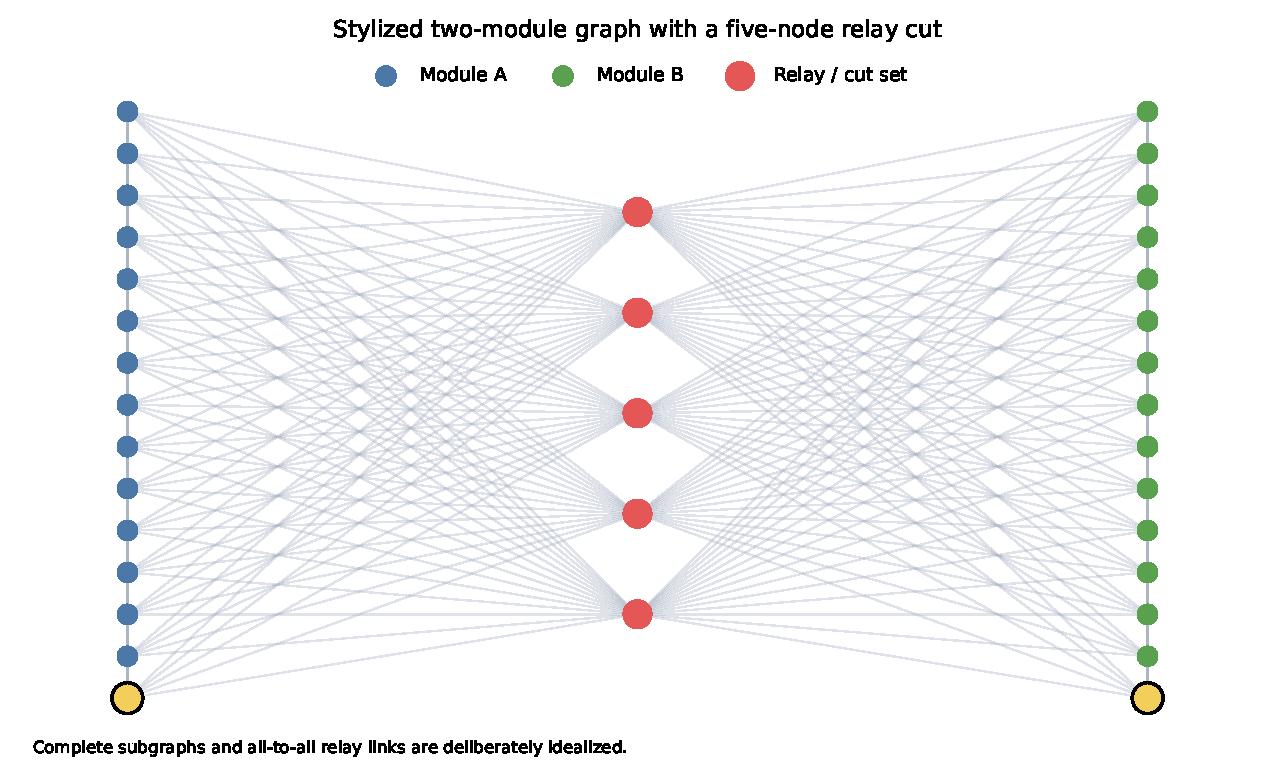
\includegraphics[width=0.86\textwidth]{fig5_structural_network.pdf}
\caption{Stylized two-module graph. The red relay vertices form an exact five-node separator between the yellow source and target anchors. The dense modules and all-to-all relay links are idealized and synthetic.}
\label{fig:network}
\end{figure}

\subsection{Experiment I: lesion placement and exact MCD}
The minimum vertex cut is computed by node splitting and max-flow/min-cut. For unit vertex cost, the computed cut consists of the five relay vertices and has capacity five. We then conduct 10,000 deletion trials for each of two random protocols. In the primary protocol, 20 vertices are sampled uniformly without replacement from all eligible non-terminal vertices, including relay nodes. In the balanced control, ten non-relay module vertices are removed from each module, while anchors and relay nodes are held fixed. A separate deterministic intervention deletes all five relay vertices.

The exact probability of disconnecting the graph under the primary random protocol is known analytically. There are 33 eligible non-terminal vertices: five relays and 28 other module vertices. Since the two anchors remain protected, the graph disconnects if and only if all five relays occur among the 20 removed vertices. Thus
\[
\Pp(\text{disconnect})=\frac{\binom{28}{15}}{\binom{33}{20}}\approx0.0653251.
\tag{22}\label{eq:hypergeom}
\]
The Monte Carlo result is compared to this exact hypergeometric probability. The result is not an estimate of biological regeneration failure; it is a test that the simulation and sampling protocol reproduce a known combinatorial probability.

\begin{figure}[H]
\centering
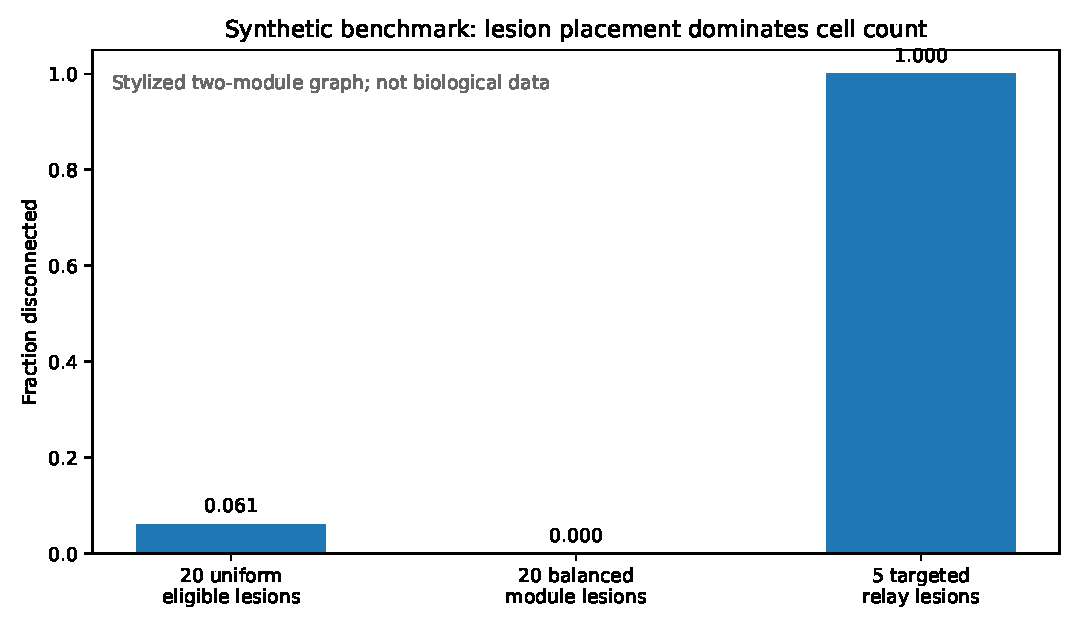
\includegraphics[width=0.78\textwidth]{fig1_lesion_topology.pdf}
\caption{Synthetic disconnection fraction under three lesion protocols. The 20-vertex uniform protocol samples relay and module vertices; the balanced protocol deliberately spares relays; the targeted protocol removes the exact cut.}
\label{fig:lesions}
\end{figure}

\begin{table}[H]
\centering\small
\caption{Experiment I: observed connectivity outcomes in the released synthetic graph.}
\begin{tabularx}{\textwidth}{p{0.31\textwidth}r r r X}
\toprule
Protocol & Trials & Failures & Fraction & Interpretation\\
\midrule
20 uniformly sampled eligible vertices & 10,000 & 612 & 0.0612 & Empirical estimate compared with exact probability 0.0653.\\
20 balanced module-cell lesions & 10,000 & 0 & 0.0000 & Relay nodes and anchors excluded by protocol.\\
5 targeted relay-node lesions & 1 & 1 & 1.0000 & Deterministic removal of the exact minimum cut.\\
\bottomrule
\end{tabularx}
\end{table}

For the 612 disconnections in 10,000 uniform trials, the Wilson 95\% interval is approximately 0.0566--0.0661 (computed by the released script). The exact probability 0.0653 lies within that interval. The balanced control exhibits no disconnections because its intervention class excludes the separator. The targeted five-node intervention disconnects the anchors by construction. The experiment therefore supports a precise statement: in this synthetic graph, connectivity depends on the placement of deleted vertices, and MCD correctly identifies the least-cost separator. It does not support the claim that 20 biological cell lesions are always recoverable or that five biological cells are a universal threshold.

\subsection{Experiment II: pinned spectral gap and diffusion}
For each relay-deletion count \(k\in\{0,1,2,3,4,5\}\), remove the first \(k\) relay vertices and compute the remaining graph Laplacian \(L_k\). Pin the source anchor with a unit diagonal penalty and compute the smallest eigenvalue of \(L_k+P\). When at least one relay survives, the graph remains connected and the pinned operator is positive definite. When all five relays are removed, the right module is disconnected from the source pin and a zero mode appears.

The numerical values for this particular graph are shown in \Cref{tab:spectral}. The positive eigenvalue is not monotone in \(k\) before disconnection. This is not a contradiction: deleting vertices changes both the operator and its dimension, and can remove slow internal relay modes while changing the coupling between modules. The theorem guarantees positive definiteness while the connected component containing the target still intersects the pin, and a zero mode when a component has no pin; it does not guarantee monotone spectral change under arbitrary node deletion.

\begin{table}[H]
\centering\small
\caption{Experiment II: smallest eigenvalue after relay vertex deletion. Values are dimensionless for the synthetic unit-weight graph.}\label{tab:spectral}
\begin{tabular}{rrrr}
\toprule
Relays removed & Relays remaining & \(\lambda_{\min}(L+P)\) & Anchors connected?\\
\midrule
0 & 5 & 0.027119 & Yes\\
1 & 4 & 0.027807 & Yes\\
2 & 3 & 0.028501 & Yes\\
3 & 2 & 0.029152 & Yes\\
4 & 1 & 0.029519 & Yes\\
5 & 0 & 0.000000 & No\\
\bottomrule
\end{tabular}
\end{table}

\begin{figure}[H]
\centering
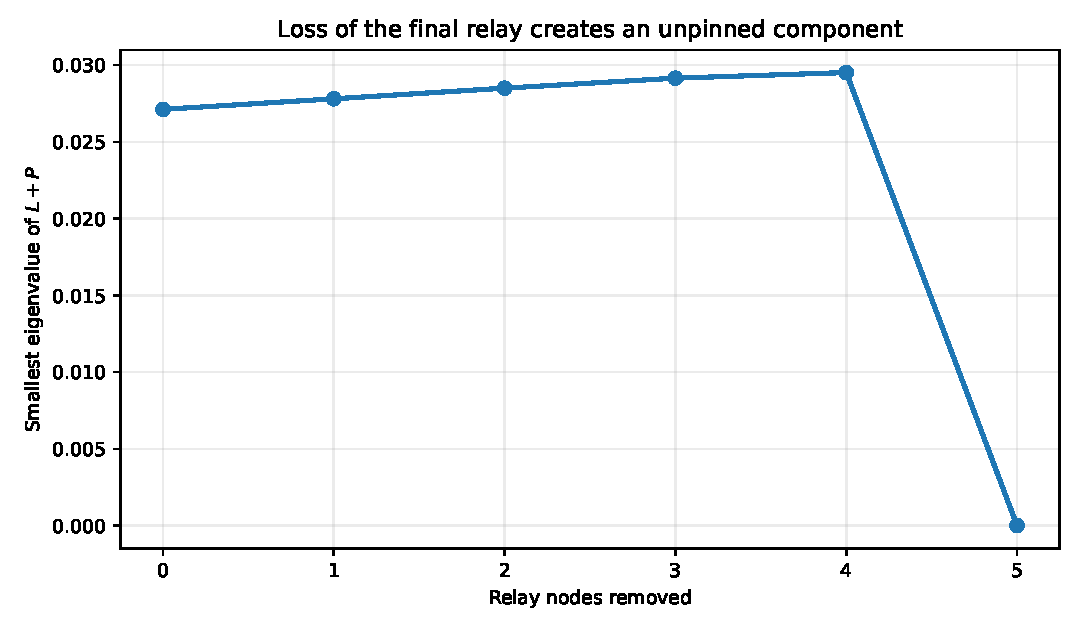
\includegraphics[width=0.79\textwidth]{fig2_pinned_spectral_gap.pdf}
\caption{Smallest eigenvalue of the pinned operator as relay vertices are removed. The finite graph exhibits non-monotone positive values before the exact disconnection produces a zero mode.}
\label{fig:spectrum}
\end{figure}

The trajectory illustration starts with a unit state in the right module and near-zero noise elsewhere, then evolves under the matrix exponential of the pinned operator. With five or one relay remaining, the right-module mean decays toward the pinned left target. With no relay, the right module is unpinned and its mean remains approximately constant after internal transients. This visual is a direct computation of the linear model, not a wound-healing trajectory.

\begin{figure}[H]
\centering
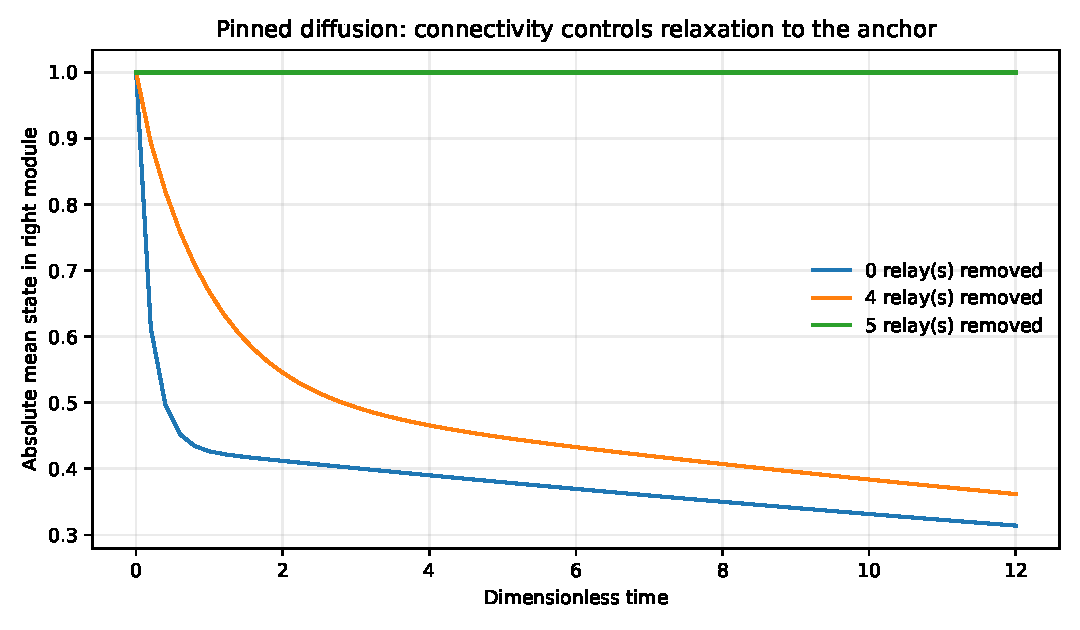
\includegraphics[width=0.79\textwidth]{fig4_pinned_diffusion_traces.pdf}
\caption{Dimensionless pinned-diffusion trajectories for zero, four, and five relay deletions. After the exact cut, the isolated module retains a neutral mean mode.}
\label{fig:traces}
\end{figure}

\subsection{Experiment III: synthetic conductance inference}
A second graph with 15 vertices and 66 candidate edges is used to keep the inverse problem computationally transparent. Two six-node cliques are connected through three relay vertices that each link to every module node. Intra-module conductances are set to one; relay-link conductances are set to 0.65. These values are simulation ground truth, not estimated biological parameters.

For each of five noise levels, 80 independent standard-normal state snapshots are generated. The forward model yields exact node derivatives under \eqref{eq:graphdiffusion}; independent zero-mean Gaussian noise is added to the derivative observations. NNLS then estimates the 66 nonnegative conductances. Five replicates are run per noise level. The design matrix has rank 66/66 and condition number approximately 4.234 in the recorded probe realization. The clean-data relative parameter error is approximately \(7.69\times10^{-16}\), i.e. floating-point precision. Mean relative error rises from 0.086\% at noise standard deviation 0.01 to 1.104\% at 0.12.

\begin{table}[H]
\centering\small
\caption{Experiment III: mean relative conductance error across five synthetic NNLS fits per noise level.}
\begin{tabular}{rrrr}
\toprule
Derivative noise SD & Mean relative error & SD across replicates & Snapshots per fit\\
\midrule
0.00 & \(7.69\times10^{-16}\) & \(1.31\times10^{-16}\) & 80\\
0.01 & 0.000860 & 0.000092 & 80\\
0.03 & 0.002608 & 0.000232 & 80\\
0.07 & 0.006321 & 0.000577 & 80\\
0.12 & 0.011035 & 0.001514 & 80\\
\bottomrule
\end{tabular}
\end{table}

\begin{figure}[H]
\centering
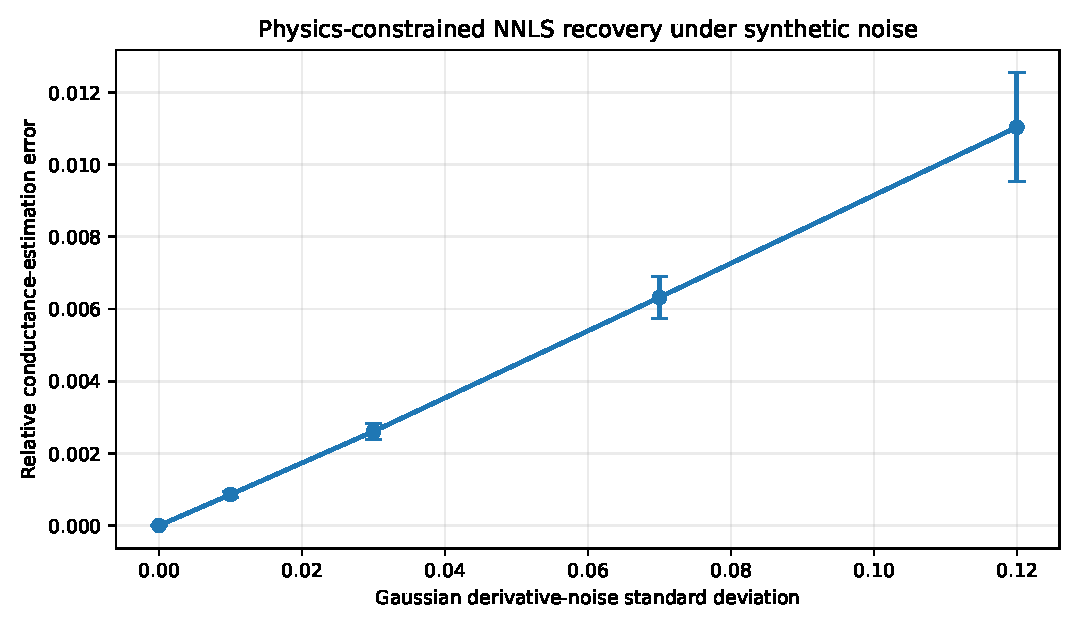
\includegraphics[width=0.79\textwidth]{fig3_nnls_noise_sensitivity.pdf}
\caption{Relative parameter-recovery error increases with derivative noise in the synthetic inverse problem. Error bars show replicate standard deviation, not a biological confidence interval.}
\label{fig:nnls}
\end{figure}

The strong recovery is expected because the candidate topology and forward law are both correct in the synthetic data generator, the state snapshots independently excite the graph, and the design matrix is well conditioned. This is a verification of the estimator under a correctly specified model. It is not evidence that real tissue conductances are identifiable from available imaging data. When the graph is wrong, the state variables are mismeasured, or important nonlinear and directed terms are omitted, NNLS may return a precise but biased graph.

\subsection{Experiment IV: sheaf exactness and cycle residual}
The four-cycle, two-dimensional stalk test yields a coboundary matrix of rank six, and therefore a first cohomology dimension of two for the graph-only complex. The exact cochain residual after harmonic projection is at numerical zero (reported in \texttt{verification\_report.json}); an independently generated random edge cochain has a nonzero harmonic part. These outputs test the quotient-space logic and protect against treating a coboundary as a nonzero cohomology class.

\begin{figure}[H]
\centering
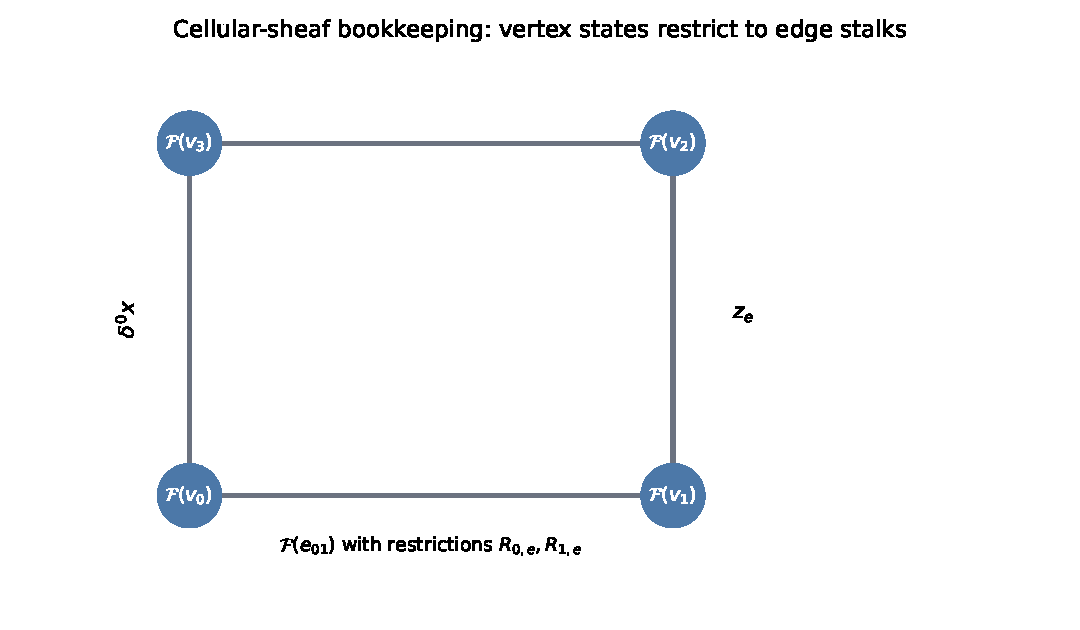
\includegraphics[width=0.76\textwidth]{fig6_sheaf_stalk_graph.pdf}
\caption{Schematic of vertex stalks, edge stalks, restriction maps, and edge-level compatibility data on a four-cycle.}
\label{fig:sheaf}
\end{figure}

\section{Sensitivity analysis and competing explanations}
\subsection{Vertex-cost sensitivity}
When all relay vertices have equal cost \(c_b\), the weighted MCD in the synthetic graph is \(5c_b\). The released code evaluates \(c_b\in\{0.25,0.5,1,2,4\}\), yielding capacities 1.25, 2.5, 5, 10, and 20 while the same five relay nodes remain the optimal cut. This is a direct consequence of the specified graph and cost model. It demonstrates that MCD is not a pure topological invariant: changing cost calibration changes the weighted distance even when the graph is unchanged.

\begin{table}[H]
\centering\small
\caption{Sensitivity of weighted MCD to the assumed cost of each relay vertex.}\label{tab:sensitivity}
\begin{tabular}{rrrr}
\toprule
Relay cost \(c_b\) & Weighted MCD & Cut cardinality & Selected vertices\\
\midrule
0.25 & 1.25 & 5 & 30--34\\
0.50 & 2.50 & 5 & 30--34\\
1.00 & 5.00 & 5 & 30--34\\
2.00 & 10.00 & 5 & 30--34\\
4.00 & 20.00 & 5 & 30--34\\
\bottomrule
\end{tabular}
\end{table}

\subsection{Graph thresholding and missing edges}
In a biological dataset, edges are not observed with certainty. An edge may be missing because a reporter is below threshold, a cell boundary is segmented incorrectly, or the chosen assay fails to detect a connection. False-positive edges can create artificial alternate paths and inflate MCD; false-negative edges can delete genuine redundancy and deflate MCD. The graph should therefore be reconstructed over a pre-specified range of thresholds, and the resulting MCD distribution reported. If the metric changes sharply under small perturbations of the segmentation or edge threshold, the result is not robust enough for biological inference.

\subsection{Alternate pathways and multilayer communication}
A bioelectric-only cut does not imply complete disconnection of the tissue. Morphogen gradients, secreted factors, extracellular matrix, mechanical stress, nervous-system inputs, and cell migration can bypass the selected graph. The appropriate model may be a multiplex graph with layer-specific costs and coupling. In that setting, the cut could remove vertices across several layers, or the model could include inter-layer edges. The choice must be driven by measured biology. A network obtained from dye transfer or gap-junction markers cannot be treated as the entire physiological network without independent evidence.

\subsection{Nonlinear dynamics and state-dependent coupling}
The linear model assumes constant edge conductances and local relaxation near a target. Biological signalling can be nonlinear, saturating, gated, time-varying, or directionally biased. If coupling depends on cell state, a conductance inferred at one voltage range may not predict another. If the system has multiple stable attractors, connectivity may allow several patterns rather than one unique target. In such settings, MCD remains a structural descriptor of the graph but the pinning theorem no longer guarantees the outcome of nonlinear dynamics.

\subsection{Counterexample: high MCD with poor function}
Consider a graph with many redundant paths but very small conductances on all edges. Its vertex cut may be large while diffusion to a pinned target is extremely slow. In a physical tissue, channels could be present but electrically ineffective, or connections could be anatomically visible while functionally gated. This counterexample shows that structural MCD cannot replace weighted dynamic measures such as relaxation time, effective resistance, or controllability metrics.

\subsection{Counterexample: low MCD with effective redundancy outside the measured layer}
Conversely, a measured gap-junction graph may have a small MCD, yet a parallel chemical or neural network may maintain the morphogenetic instruction. The selected graph would be fragile but the organism might still regenerate. This does not falsify graph cut mathematics; it falsifies the claim that the selected graph is a complete representation of the relevant communication task.

\subsection{Why curvature and non-Hermitian effects are not core variables here}
The motivating concept proposed assigning negative Ollivier--Ricci curvature to a bottleneck and using a non-Hermitian skin-effect operator to direct repair. These mechanisms were not retained in the core model. Graph curvature depends on the metric and transport measures chosen and is not, by itself, a minimum cut or causal measure of tissue vulnerability. Non-Hermitian localization requires a specified non-reciprocal operator, boundary conditions, and spectral evidence; it cannot be inferred merely from the existence of a wound edge. The released model uses exact cut computation and a symmetric Laplacian precisely because those objects have transparent definitions and independent checks.

\begin{table}[H]
\centering\small
\caption{Competing explanations and discriminating evidence.}
\begin{tabularx}{\textwidth}{p{0.25\textwidth}p{0.35\textwidth}X}
\toprule
Explanation & What it predicts & Evidence that distinguishes it from a pure cut model\\
\midrule
Graph-cut vulnerability & Outcome tracks pre-registered weighted separator cost after controlling lesion burden. & Matched lesion-count interventions at distinct graph positions; independent graph reconstruction.\\
Local cell-loss / viability & Outcome tracks cell death, wound size, or proliferation impairment rather than connectivity. & Viability and proliferation covariates; rescue controls that restore cells without restoring edges.\\
Parallel signalling layers & A cut in one measured layer does not interrupt the total morphogenetic command. & Simultaneous measurements or perturbations of electrical, chemical, neural, and mechanical channels.\\
Nonlinear state memory & Persistent state depends on attractor basin and prior history, not only graph separation. & Longitudinal pre-injury and post-injury state measurements; repeated regeneration assays.\\
Measurement artefact & Apparent bottleneck is caused by segmentation or threshold selection. & Blinded multi-annotator graph reconstruction, threshold sweeps, and independent modalities.\\
\bottomrule
\end{tabularx}
\end{table}

\section{Prospective biological validation programme}
\subsection{Design principle}
The next meaningful study is not to apply a presumed therapy or to infer a universal law from another toy simulation. It is to measure a communication graph before injury, predefine source and target regions, quantify graph uncertainty, and then compare lesion patterns with similar cell counts but different predicted MCD. A positive result would require MCD to predict an outcome beyond ordinary lesion size, location, viability, and known molecular determinants. A null result would be equally informative if the graph was adequately measured.

\subsection{Measurement layer}
A candidate planarian experiment could combine a cell-resolved anatomical segmentation with a validated assay for intercellular coupling, voltage-sensitive measurements, and a time-resolved record of early wound responses. The exact assay should be selected by domain experts based on species, instrumentation, toxicity, and existing validated protocols. The graph should be generated using a pre-registered edge rule, and the state variables and restriction maps should be specified without reference to later regeneration outcomes.

The measurement team should distinguish structural adjacency from functional coupling. Physical contact does not necessarily imply effective electrical communication; conversely, an effective signal can pass through a route not captured by a simple adjacency graph. Independent modality comparisons are necessary. Each cell and link should carry uncertainty or confidence rather than being forced into a binary call when the assay is ambiguous.

\subsection{Perturbation design}
Where ethically and technically justified, compare matched perturbations that differ in their predicted network effect. One arm should use spatially dispersed targets, another should target a precomputed separator, and a control should include sham or non-network perturbation. Interventions should be matched as closely as possible for total cell loss, tissue damage, wound geometry, and viability. The study should not define the separator retrospectively from the observed phenotype.

The relevant outcome should not be only immediate wound closure. It may include the fidelity of regenerated anterior--posterior polarity, the proportion and timing of anatomical outcomes, and reproducibility after a subsequent regeneration cycle. Because prior work reports persistent and latent patterning states, longitudinal follow-up can be important \citep{Durant2017,Durant2019}. However, the protocol must be developed and approved by the relevant biological team; this paper supplies a design logic, not a validated wet-lab procedure.

\subsection{Pre-registration and analysis}
Before data collection, register: species and strain, segmentation method, assay modality, source/target anchors, candidate graph edges, restriction maps, cost definition, cut algorithm, primary outcome, covariates, exclusion criteria, and statistical test. Estimate MCD on the baseline graph only. Then compare it with outcomes using a model that includes lesion count, lesion geometry, viability, and other measured covariates. The primary analysis should test whether MCD adds predictive information beyond those variables, with cross-validation at the animal or experimental-batch level to avoid leakage.

Uncertainty in graph reconstruction should propagate into the outcome model. One approach is to sample plausible graphs from calibrated edge probabilities and calculate an MCD distribution for each specimen. Another is to report bounds under conservative and permissive edge thresholds. A single best-fit graph can be retained for interpretability, but should not be the only basis of inference.

\subsection{Falsification criteria}
The central biological hypothesis should be rejected or substantially revised if any of the following occurs:
\begin{enumerate}
\item MCD does not predict regeneration outcomes after controlling for lesion count, geometry, viability, and established molecular covariates.
\item Repeatedly deleting the predicted separator does not impair the chosen communication task, despite adequate target engagement and validated graph reconstruction.
\item Lesions with higher predicted MCD fail at equal or greater rates than lower-MCD matched lesions, with confidence intervals excluding a useful effect size.
\item The inferred graph is unstable under reasonable segmentation or assay thresholds, and MCD changes more than the outcome association can tolerate.
\item A parallel signalling layer explains recovery better than the selected communication graph.
\item The linearized diffusion model produces structured residuals or fails to predict response outside the fitted perturbation regime.
\end{enumerate}

\begin{figure}[H]
\centering
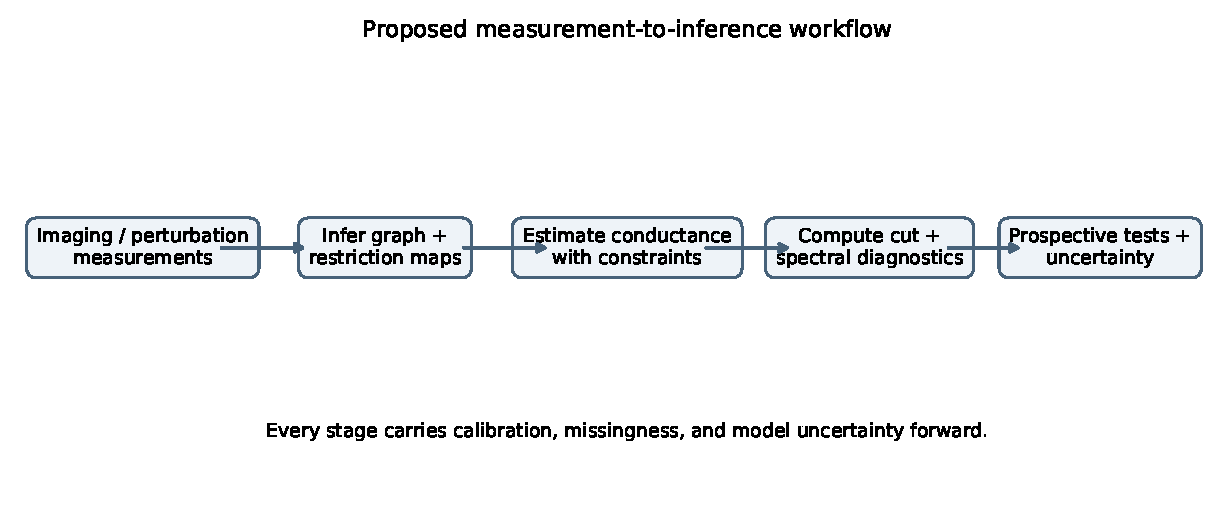
\includegraphics[width=0.88\textwidth]{fig7_inference_flow.pdf}
\caption{Proposed computational pipeline from measurements to network inference, MCD calculation, and prospective validation. All stages retain uncertainty and calibration metadata.}
\label{fig:workflow}
\end{figure}

\begin{figure}[H]
\centering
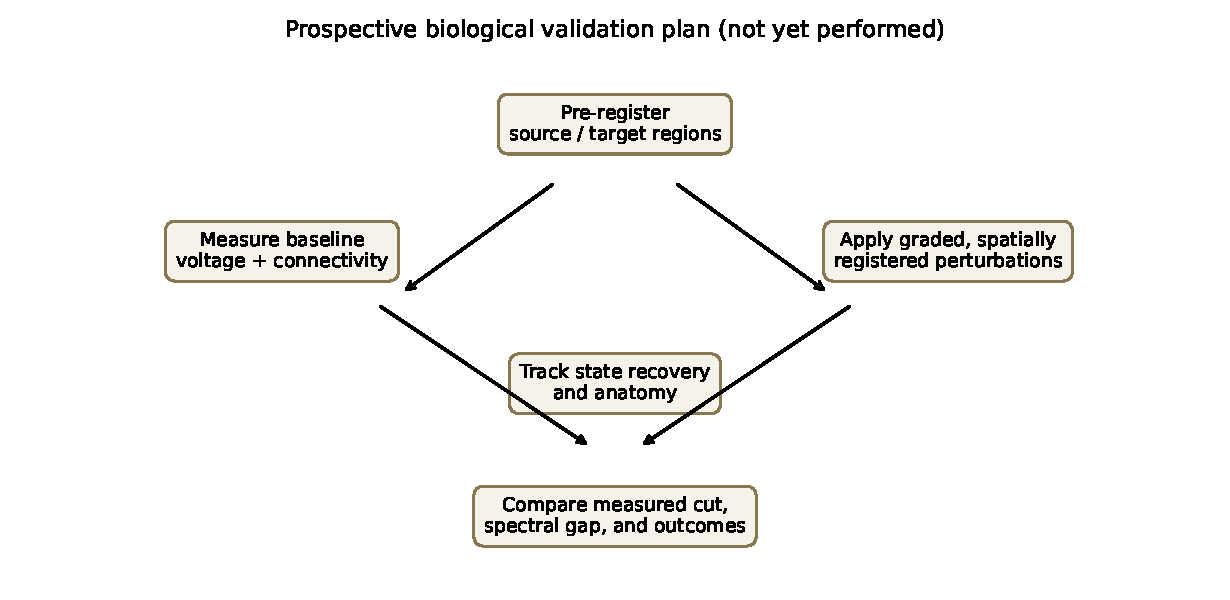
\includegraphics[width=0.88\textwidth]{fig8_validation_flow.pdf}
\caption{Prospective biological validation logic. The flow is a proposal only; no wet-lab experiment is reported in this paper.}
\label{fig:wetlab}
\end{figure}

\section{Comparative screening of research directions}
The original conceptual programme included multiple ambitious directions: a universal fault-tolerant persistence law, biological quantum error correction, sheaf-theoretic tissue compatibility, non-Hermitian wound localization, spin-glass ageing, anyon condensation in cancer, and holographic bulk reconstruction. These directions were not treated as established results. They were compared as possible research contributions and narrowed to the most operationally testable question.

\begin{table}[H]
\centering\scriptsize
\caption{Internal scope-screening of ten candidate contributions. Scores are reasoned editorial ratings from 1 (weak) to 5 (strong), not external peer-review assessments. The selected line is the operational network-resilience framework.}\label{tab:candidates}
\begin{tabularx}{\textwidth}{p{0.22\textwidth}rrrrrrX}
\toprule
Candidate & Signif. & Math. & AI role & Testability & Falsif. & Credibility & Decision\\
\midrule
Universal fault-tolerant persistence across life and spacetime & 5 & 2 & 1 & 1 & 1 & 1 & Reject: too broad; cross-domain analogy is not a unified mechanism.\\
Biological tissue as a literal quantum stabilizer code & 4 & 3 & 1 & 1 & 2 & 1 & Reject as literal claim: no biological code space or logical operators defined.\\
MCD as weighted source--target vertex cut & 4 & 5 & 3 & 5 & 5 & 4 & Select: exact, reproducible, experimentally falsifiable once a graph is measured.\\
Hodge residuals for tissue compatibility data & 3 & 5 & 3 & 4 & 5 & 4 & Retain as a complementary diagnostic, not an independent biological mechanism.\\
Non-Hermitian skin effect as wound-edge repair engine & 3 & 3 & 2 & 2 & 3 & 2 & Defer: requires measured non-reciprocity and a validated operator.\\
Spin-glass frustration as a quantitative ageing law & 4 & 3 & 2 & 2 & 3 & 2 & Defer: no ageing dynamics or calibrated frustration variable in the supplied model.\\
Anyon condensation as a cancer mechanism & 5 & 2 & 1 & 1 & 2 & 1 & Reject as mechanism: presently a metaphor without biological anyonic degrees of freedom.\\
AI inverse estimation of tissue communication weights & 4 & 4 & 5 & 4 & 5 & 4 & Retain as the measurable data-to-graph component; method itself is not claimed novel.\\
Bioelectric optimal control of regenerative polarity & 4 & 4 & 3 & 3 & 4 & 3 & Defer until graph and state parameters are experimentally identified.\\
Holographic reconstruction of internal organs from epithelial boundary codes & 3 & 2 & 1 & 1 & 2 & 1 & Reject from current paper: no defensible map from tissue data to AdS/CFT reconstruction.\\
\bottomrule
\end{tabularx}
\end{table}

The selected scope is intentionally less grand than the original title, but it creates a chain of verifiable objects: data, graph, cost model, minimum cut, sheaf compatibility, linear stability, and inverse-estimation error. A more expansive theory should be earned by new data and theorems rather than by adding disciplinary terminology.

\section{Limitations and unresolved mathematical questions}
\subsection{No measured biological graph}
The principal limitation is the absence of an experimentally measured tissue graph. The synthetic graph's cliques, relays, and unit capacities were selected to illustrate a precise theorem. They do not represent measured planarian tissue geometry, innexin expression, gap-junction conductance, or voltage propagation. The reported 5.0 cut is a model output for the constructed graph only.

\subsection{Static graph assumption}
Cellular networks change with injury, migration, proliferation, and differentiation. A static graph may be reasonable only over a narrow time interval. Dynamic graphs \(G(t)\) or temporal networks may be required if links are gained and lost during regeneration. In such a model, MCD could be defined over time-respecting paths, but the exact definition and algorithm would need separate development.

\subsection{Directed, signed, and non-reciprocal links}
The core theory assumes an undirected graph and symmetric positive weights. If directed signalling is measured, a directed vertex cut still exists, but the Laplacian and stability analysis change. If links can be inhibitory or sign-changing, the positive-semidefinite energy structure may fail unless the model is reformulated as a connection or signed Laplacian with explicit assumptions. Non-Hermitian operators should be introduced only after directional coupling is actually measured.

\subsection{Sheaf construction is not automatic}
The use of the word sheaf does not by itself create a biological model. Stalks, restriction maps, cochains, face maps, and measurement units must be specified. An identity-restriction constant sheaf may be a useful first approximation, but it cannot encode arbitrary spatially varying target patterns without offsets or a richer sheaf. A higher-dimensional complex must enforce \(\delta^1\delta^0=0\). Future work should compare trivial sheaves with biologically motivated vector bundles, connection sheaves, and empirical restriction maps.

\subsection{MCD does not equal dynamical robustness}
A minimum vertex cut only addresses disconnection under node removal. It does not account for edge weakening, signal delay, nonlinear thresholds, stochastic switching, cell replacement, feedback, or repair capacity. A tissue with high MCD may still be dynamically fragile; a tissue with low MCD may compensate through unmeasured pathways. MCD should therefore be reported alongside conductance-weighted spectral quantities, effective resistance, and direct functional endpoints.

\subsection{No empirical claims about ageing or cancer}
The present work does not study ageing or cancer. It does not derive a monotone decrease of MCD with age, a spin-glass mechanism, a cancer phase transition, or a bioelectric treatment effect. The supplied earlier simulation suite assigned cohort parameters and intervention outputs by explicit formulas, including preset post-intervention values; those outputs cannot be interpreted as independently generated biological evidence. A valid future model would need a specified stochastic ageing process or tumour dynamics, calibrated parameters, independent data, and tests against competing mechanisms. This paper deliberately removes these unsupported results.

\subsection{Inference-model limitations}
The synthetic inverse problem assumes the candidate edge set is known and the forward equation is correct. It uses randomly generated independent state snapshots, exact derivatives, and additive Gaussian measurement noise. It does not model observation noise in the state variables, derivative estimation from time series, correlated noise, edge uncertainty, hidden nodes, time-varying couplings, or nonlinear biological regulation. The NNLS output is not a validated estimator for real tissue until evaluated on appropriate data.

\subsection{Open mathematical questions}
Several questions remain. First, can a weighted MCD distribution be bounded under graph uncertainty in a way that remains computationally tractable for large cellular networks? Second, can a multiplex cut be defined that allows distinct costs for electrical, chemical, mechanical, and neural pathways without double-counting cells? Third, what conditions relate the graph cut to a controllability or observability measure for the linearized morphogenetic dynamics? Fourth, how should affine sheaf sections encode spatially varying anatomical targets and wound-dependent boundary conditions? Fifth, can an experimentally meaningful cost function be calibrated independently of outcome labels? These are distinct problems and should not be collapsed into a single scalar without justification.

\section{Discussion}
The central conceptual shift is from a biological metaphor of error correction to an operational network question. If the tissue-level task is to communicate a patterning signal between two regions, how many independent routes exist, and what is the least costly set of cells whose loss eliminates every route? The MCD definition provides an exact answer for a measured graph and a specified task. This can help design experiments in which lesion burden is held approximately fixed while lesion placement varies relative to the graph's separator structure.

The formalism's strongest feature is its separation of three different diagnostics. The cut metric measures the minimum vertex removal cost for source--target disconnection. The sheaf Laplacian measures compatibility energy and provides a linear relaxation operator. The harmonic residual measures the portion of observed edge data that cannot be represented as an exact vertex-level difference under the chosen sheaf. These quantities are related but not interchangeable. A paper that reports all three must retain their distinct meanings.

The pinning theorem is a simple but useful bridge between topology and dynamics. It states that a positive-semidefinite compatibility operator can have neutral modes, and that anchors remove those modes only if they intersect every compatible component. In ordinary graph diffusion, a connected component with no anchor retains a constant mode. This is the exact mathematical meaning of the zero eigenvalue displayed in the synthetic experiment. It does not imply that a living tissue's cells will fail to regenerate after a corresponding lesion, because real tissues have multiple signalling layers and nonlinear feedback.

The AI component is likewise intentionally modest. A model-informed inverse estimator is necessary to turn a measured communication system into weights, but the numerical result is meaningful only if the forward model is identifiable and its assumptions survive empirical tests. A black-box predictor that maps a static image directly to regeneration success would not answer the same question. The proposed pipeline keeps the chain interpretable: measurement to candidate graph, graph to conductance estimates, conductances to cuts and spectra, and those quantities to prospective outcomes.

In a biological study, the best outcome would not be a high correlation between MCD and regeneration in one dataset. It would be a preregistered and independently replicated predictive relationship that improves on lesion count, lesion geometry, cell viability, and known molecular markers. A particularly informative result would be a matched perturbation comparison in which a lower cell count but a lower MCD lesion produces a larger, reproducible functional effect than a more dispersed lesion, after alternate communication routes have been measured. Conversely, failure of MCD to add predictive value would delimit the role of network cuts in morphogenesis.

\section{Conclusion}
We introduced a model-relative Morphogenetic Code Distance defined as a weighted minimum vertex cut between prescribed source and target regions of a communication graph. We placed this metric in a finite-dimensional cellular-sheaf framework, derived the associated positive-semidefinite Laplacian, proved a pinning criterion for exponential convergence, and formalized the distinction between exact coboundary residuals and nontrivial cohomological obstructions. We also specified a physics-constrained NNLS procedure for estimating nonnegative edge conductances and audited its rank and noise sensitivity on a synthetic inverse problem.

The computational benchmark confirms only the mathematics and software behavior that it explicitly tests: the weighted cut is five for the constructed graph; random lesion outcomes agree with the exact hypergeometric baseline; targeted relay removal disconnects the designated anchors; the pinned operator has a zero mode when an unpinned component is created; and NNLS recovers known synthetic parameters under the specified excitation and noise model. None of these outcomes establishes a biological MCD, validates a planarian regeneration mechanism, or provides evidence for ageing reversal or cancer normalization.

The next step is measurement, not further metaphor. A biological application requires a calibrated cell-resolved communication graph, independently specified stalks and restriction maps, uncertainty-aware conductance inference, matched perturbations, and a falsification-first analysis. If those tests succeed, MCD may become a useful quantitative descriptor of morphogenetic network resilience. If they fail, the definitions remain mathematically valid while the proposed biological mapping must be revised.

\section*{Research-process disclosure}
Co-equal research-process credit is given to Devanik Debnath and Xylia, the autonomous multi-model research engine coordinating AI-assisted discovery, synthesis, and verification. Devanik Debnath retains responsibility for the final manuscript, scientific claims, citations, and released artifacts.

\section*{Data and code availability}
All synthetic data, figure-generation code, verification routines, and result summaries for this preprint are included in the accompanying release directory. Run \texttt{python verify\_model.py} from that directory to regenerate the numerical outputs and figures. No biological dataset was generated or analyzed. The exact software versions used in the recorded run are stored in \texttt{results/verification\_report.json}. The present GitHub archive is a source-and-evidence release, not a peer-reviewed publication or a Zenodo deposit.

\appendix
\section{Proof details and algebraic identities}
\subsection{Positive semidefiniteness of the sheaf Laplacian}
Let \(W\succ0\) and let \(D\) be the matrix of \(\delta^0\). The matrix \(L_0=D^*WD\) is self-adjoint because \(W\) is self-adjoint. For any vector \(x\),
\[
x^*L_0x=x^*D^*WDx=(Dx)^*W(Dx)=\norm{W^{1/2}Dx}_2^2\geq0.
\]
Therefore all eigenvalues of \(L_0\) are real and nonnegative. The kernel is \(\ker L_0=\ker D\) when \(W\succ0\), because zero quadratic energy is equivalent to \(Dx=0\). This identity is P1 and does not require a biological interpretation.

\subsection{Kernel of the pinned operator}
The same argument gives
\[
\ker(L_0+P)=\ker L_0\cap\ker P
\]
for positive-semidefinite self-adjoint operators in finite dimensions. To see this, if \((L_0+P)x=0\), then its quadratic form is zero. Both nonnegative terms must vanish separately. Conversely, any vector in both kernels is in the sum's kernel. The criterion in Theorem 1 follows.

\subsection{Exponential decay}
For the ODE \(\dot y=-Ay\), the exact solution is \(y(t)=e^{-At}y(0)\). If \(A\succ0\) is self-adjoint, its spectral decomposition has eigenvalues \(\lambda_i\geq\lambda_{\min}>0\). Thus
\[
\norm{e^{-At}}_2=\max_i e^{-\lambda_i t}=e^{-\lambda_{\min}t},
\]
which yields the bound in Eq. (15). If \(A\) has a zero eigenvalue, the operator norm of \(e^{-At}\) remains one, and components along the kernel need not decay.

\subsection{Exact vertex cut as a flow problem}
For an eligible node \(v\), the split edge \(v_{\mathrm{in}}\to v_{\mathrm{out}}\) carries capacity \(c_v\). Any path through the original vertex must traverse that split edge. A cut crossing the split edge corresponds to deleting the original vertex. Original graph edges and protected anchors receive capacity \(M\), chosen larger than the total finite cost of deleting all eligible vertices. Therefore no minimum cut uses an original edge or protected anchor, and the min-flow/min-cut value equals the minimum total vertex-removal cost. This proves correctness of the construction used in the code for finite graphs with positive costs.

\subsection{Exact probability for the uniform deletion protocol}
The structural benchmark has 35 vertices. Two are protected terminals, leaving 33 eligible vertices, of which five are relay vertices. The uniform protocol samples 20 eligible vertices without replacement. The anchor-to-anchor path remains if and only if at least one relay survives. The failure event is that all five relay vertices are included among the 20 removed vertices. Once those five are fixed, the remaining 15 removals must be chosen from the 28 non-relay eligible vertices. The total number of equally likely 20-subsets is \(\binom{33}{20}\), so the exact failure probability is Eq. (22). This analytic value is used as an independent reference for the Monte Carlo result.

\section{Algorithmic details and computational complexity}
\subsection{Minimum vertex cut}
The node-splitting construction doubles the number of graph vertices and adds one split edge per node plus two directed arcs per undirected edge. The exact max-flow runtime depends on the chosen flow algorithm and graph structure. The released implementation uses NetworkX's minimum-cut routine and is intended for reproducibility and moderate synthetic graphs. Large tissue-scale graphs may require specialized sparse flow solvers, graph partitioning heuristics, or repeated local-cut algorithms. Any approximation must be labelled and its gap from an exact solution estimated on tractable subproblems.

\subsection{Sheaf matrix assembly}
For a constant \(d\)-dimensional stalk with identity restrictions, each oriented edge contributes a \(d\times d\) identity block to the tail vertex columns and a negative identity block to the head columns. The resulting coboundary matrix is sparse, with two nonzero blocks per edge. For general sheaves, the blocks are the measured or specified restriction maps. The Laplacian should be constructed from this sparse operator rather than by manually assigning eigenvalues or curvature labels.

\subsection{NNLS implementation}
The released code assembles one row per node per state snapshot. For an edge \(e=(u,v)\), the column corresponding to that edge has value \(x_u-x_v\) in the row for node \(u\), value \(x_v-x_u\) in the row for node \(v\), and zero elsewhere. The response is the negative derivative. The optimizer is SciPy's nonnegative least-squares routine. The design rank and singular-value condition number are computed on a probe realization, and every noise level is evaluated across five deterministic replicates.

\subsection{Reproducibility and failure behavior}
A fixed pseudo-random seed is set in the script. The script tests invalid source/sink combinations and non-positive node capacities, verifies the Laplacian energy identity, checks exact cochain projection, checks the minimum cut, tests a known hypergeometric deletion probability, computes the pinned spectral gap, and tests NNLS recovery under clean and noisy synthetic conditions. Required assertions raise an exception and cause a nonzero process exit. Outputs are written relative to the script location, so the program can be run from an unrelated current working directory.

\section{Claim--evidence matrix}
\setlength{\tabcolsep}{3pt}
\footnotesize
\begin{longtable}{@{}p{0.31\textwidth}p{0.10\textwidth}p{0.24\textwidth}p{0.25\textwidth}@{}}
\caption{Claim--evidence matrix for the release.}\label{tab:claims}\\
\toprule
Claim & Level & Evidence in this paper & Residual requirement\\
\midrule
\endfirsthead
\toprule
Claim & Level & Evidence in this paper & Residual requirement\\
\midrule
\endhead
The weighted sheaf Laplacian is positive semidefinite. & P1 & Algebraic identity and numerical energy check. & None for the stated finite-dimensional assumptions.\\
An exact coboundary has zero class in \(H^1\). & P1 & Quotient definition, Hodge projection, and four-cycle test. & Higher-dimensional complexes require a consistent \(\delta^1\).\\
The node-splitting flow equals weighted vertex cut. & P1 & Construction proof and exact synthetic graph result. & Validate implementation on independent graph libraries for large instances.\\
A connected ordinary graph with a positive pin has a positive pinned gap. & P1/P2 & Kernel criterion and finite-dimensional proof. & Biological dynamics may not be symmetric or linear.\\
Five relay nodes form the MCD in the toy graph. & P1 & Exact min-cut value 5; cut nodes 30--34. & No biological transfer is implied.\\
Twenty random deletions fail with probability near 6.53\%. & Synthetic statistical check & 612/10,000 compared with exact hypergeometric probability. & The probability is specific to this graph and sampling rule.\\
NNLS recovers 66 synthetic weights under 80 snapshots. & Synthetic numerical result & Full-rank design and recorded noise sweep. & Real measurement noise, hidden nodes, and model misspecification remain untested.\\
Planarian polarity involves bioelectric and neural cues. & Empirical literature & Primary studies cited in Sec. 2. & Does not validate MCD or a sheaf model.\\
MCD predicts anatomical regeneration success. & P3 hypothesis & No biological test in this release. & Requires preregistered experiments and independent replication.\\
Tissue is a literal quantum error-correcting code. & P5 / unsupported & Not claimed. & Would require explicit code space, stabilizers, logical operators, and measurements.\\
\bottomrule
\end{longtable}
\normalsize
\setlength{\tabcolsep}{6pt}

\section{Release contents and verification record}
The accompanying release contains the nine core files required by the research archive and the \texttt{figures/} and \texttt{results/} evidence directories. The figures comprise four numerical plots, two structural graph illustrations, and two process/validation flow diagrams. The result directory stores data tables for the Monte Carlo, spectral, inference, trajectory, and cost-sensitivity computations, along with JSON verification results, environment information, and content hashes. The verification summary records passed mathematical and synthetic checks separately from untested biological claims.

The release uses no downloaded biological dataset and no personally identifiable research participant data. Re-running the script should regenerate the synthetic outputs and figures. Exact byte-for-byte PDF reproducibility may depend on the LaTeX engine and font package versions, which should be recorded by the build pipeline. The repository commit and release tag, if available, are archival identifiers only; they do not imply peer review, a journal publication, or an issued DOI.

\begin{thebibliography}{99}
\footnotesize
\setlength{\itemsep}{1pt}
\setlength{\parskip}{0pt}
\bibitem[Brunton et~al.(2016)Brunton, Proctor, and Kutz]{Brunton2016}
Brunton, S. L., Proctor, J. L., and Kutz, J. N. (2016).
Discovering governing equations from data by sparse identification of nonlinear dynamical systems.
\emph{Proceedings of the National Academy of Sciences}, 113(15), 3932--3937.
\href{https://doi.org/10.1073/pnas.1517384113}{doi:10.1073/pnas.1517384113}.

\bibitem[Chung(1997)]{Chung1997}
Chung, F. R. K. (1997). \emph{Spectral Graph Theory}.
CBMS Regional Conference Series in Mathematics, Vol. 92.
American Mathematical Society, Providence, RI.
\href{https://doi.org/10.1090/cbms/092}{doi:10.1090/cbms/092}.

\bibitem[Durant et~al.(2016)Durant, Lobo, Hammelman, and Levin]{Levin2016Patterning}
Durant, F., Lobo, D., Hammelman, J., and Levin, M. (2016).
Physiological controls of large-scale patterning in planarian regeneration: A molecular and computational perspective on growth and form.
\emph{Regeneration}, 3(2), 78--102.
\href{https://doi.org/10.1002/reg2.54}{doi:10.1002/reg2.54}.

\bibitem[Durant et~al.(2017)Durant et~al.]{Durant2017}
Durant, F., Morokuma, J., Fields, C., Williams, K., Adams, D. S., and Levin, M. (2017).
Long-term, stochastic editing of regenerative anatomy via targeting endogenous bioelectric gradients.
\emph{Biophysical Journal}, 112(10), 2231--2243.
\href{https://doi.org/10.1016/j.bpj.2017.04.011}{doi:10.1016/j.bpj.2017.04.011}.

\bibitem[Durant et~al.(2019)Durant et~al.]{Durant2019}
Durant, F., Bischof, J., Fields, C., Morokuma, J., LaPalme, J., Hoi, A., and Levin, M. (2019).
The role of early bioelectric signals in the regeneration of planarian anterior/posterior polarity.
\emph{Biophysical Journal}, 116(5), 948--961.
\href{https://doi.org/10.1016/j.bpj.2019.01.029}{doi:10.1016/j.bpj.2019.01.029}.

\bibitem[Ford and Fulkerson(1956)]{FordFulkerson1956}
Ford, L. R., Jr., and Fulkerson, D. R. (1956).
Maximal flow through a network.
\emph{Canadian Journal of Mathematics}, 8, 399--404.
\href{https://doi.org/10.4153/CJM-1956-045-5}{doi:10.4153/CJM-1956-045-5}.

\bibitem[Hansen and Ghrist(2019)]{HansenGhrist2019}
Hansen, J., and Ghrist, R. (2019).
Toward a spectral theory of cellular sheaves.
\emph{Journal of Applied and Computational Topology}, 3, 315--358.
\href{https://doi.org/10.1007/s41468-019-00038-7}{doi:10.1007/s41468-019-00038-7}.

\bibitem[Kitaev(2003)]{Kitaev2003}
Kitaev, A. Y. (2003).
Fault-tolerant quantum computation by anyons.
\emph{Annals of Physics}, 303(1), 2--30.
\href{https://doi.org/10.1016/S0003-4916(02)00018-0}{doi:10.1016/S0003-4916(02)00018-0}.

\bibitem[Levin(2021)]{Levin2021}
Levin, M. (2021).
Bioelectric signaling: Reprogrammable circuits underlying embryogenesis, regeneration, and cancer.
\emph{Cell}, 184(8), 1971--1989.
\href{https://doi.org/10.1016/j.cell.2021.02.034}{doi:10.1016/j.cell.2021.02.034}.

\bibitem[Lim(2020)]{Lim2020}
Lim, L.-H. (2020).
Hodge Laplacians on graphs.
\emph{SIAM Review}, 62(3), 685--715.
\href{https://doi.org/10.1137/18M1223101}{doi:10.1137/18M1223101}.

\bibitem[Oviedo et~al.(2010)Oviedo et~al.]{Oviedo2010}
Oviedo, N. J., Morokuma, J., Walentek, P., Kema, I. P., Gu, M. B., Ahn, J.-M., Hwang, J. S., Gojobori, T., and Levin, M. (2010).
Long-range neural and gap junction protein-mediated cues control polarity during planarian regeneration.
\emph{Developmental Biology}, 339(1), 188--199.
\href{https://doi.org/10.1016/j.ydbio.2009.12.012}{doi:10.1016/j.ydbio.2009.12.012}.

\bibitem[Reddien and S\'anchez Alvarado(2004)]{Reddien2004}
Reddien, P. W., and S\'anchez Alvarado, A. (2004).
Fundamentals of planarian regeneration.
\emph{Annual Review of Cell and Developmental Biology}, 20, 725--757.
\href{https://doi.org/10.1146/annurev.cellbio.20.010403.095114}{doi:10.1146/annurev.cellbio.20.010403.095114}.

\bibitem[Shandilya and Timme(2011)]{ShandilyaTimme2011}
Shandilya, S. G., and Timme, M. (2011).
Inferring network topology from complex dynamics.
\emph{New Journal of Physics}, 13, 013004.
\href{https://doi.org/10.1088/1367-2630/13/1/013004}{doi:10.1088/1367-2630/13/1/013004}.
\end{thebibliography}
\end{document}